\documentclass[12pt]{article}
\usepackage[a4paper, total={6in, 10in}]{geometry}
%\usepackage[utf8]{inputenc}

\usepackage{amsmath, amsfonts, amssymb, amsthm}
\usepackage[scr=dutchcal]{mathalpha}

\usepackage{hyperref}
\hypersetup{
    colorlinks=true,
    linkcolor=blue,
    urlcolor=blue
}
\usepackage{indentfirst}

\usepackage{xeCJK}
\usepackage{fontspec}
\usepackage{xcolor}
\definecolor{codegreen}{rgb}{0,0.6,0}
\definecolor{codegray}{rgb}{0.5,0.5,0.5}
\definecolor{codepurple}{rgb}{0.58,0,0.82}
\definecolor{backcolour}{rgb}{0.95,0.95,0.92}

\usepackage{graphicx}
\usepackage{float}
\usepackage{booktabs}

\usepackage{caption}
\usepackage{subcaption}

\usepackage{fancyvrb}
\usepackage{fancyhdr, lastpage}
\usepackage{verbatim}

\usepackage{algorithm}
\usepackage{algpseudocode}
\usepackage{listings}
\lstdefinestyle{mystyle}{
    backgroundcolor=\color{backcolour},   
    commentstyle=\color{codegreen},
    keywordstyle=\color{magenta},
    numberstyle=\tiny\color{codegray},
    stringstyle=\color{codepurple},
    basicstyle=\ttfamily\small,
    breakatwhitespace=false,         
    breaklines=true,                 
    captionpos=b,                    
    keepspaces=true,                 
    numbers=left,                    
    numbersep=5pt,                  
    showspaces=false,                
    showstringspaces=false,
    showtabs=false,                  
    tabsize=2
}

\usepackage{mathtools}
\usepackage{tikz}
\usepackage{tcolorbox}

\usepackage{biblatex}
\addbibresource{reference.bib}

\usepackage{siunitx}
\usepackage{setspace}
\usepackage{lipsum}
\usepackage{enumerate}

\newtheorem{theorem}{Theorem}[subsection]
\newtheorem{corollary}{Corollary}[theorem]
\newtheorem{lemma}[theorem]{Lemma}
\theoremstyle{definition}
\newtheorem{definition}[theorem]{Definition}
\newtheorem{proposition}[theorem]{Proposition}
\newtheorem{example}[theorem]{Example}

\newcommand{\colvec}[2][0.8]{
  \scalebox{#1}{
    \renewcommand{\arraystretch}{.8}
    $\begin{bmatrix}#2\end{bmatrix}$
  }
}

\setCJKmainfont{AR PL UKai TW}
\renewcommand{\baselinestretch}{1.25}
\setlength{\parindent}{2em}
%%%%%%%%%%%%%%%%%%%%%%%%%%%%%%
\begin{document}

\title{
    \Large A Singular Value Decomposition Approach to Image Compression and Live Photo Processing \\
    \large 112-1 Introduction to Scientific Computation (I) Final Project
}
\author{
    $\quad$林宜亭$\quad$ \and
    $\quad$黃俊袺$\quad$ \and
    $\quad$江信彥$\quad$ \and
    $\quad$黃建富$\quad$ \and
    $\quad$林呂約$\quad$ \and
    $\quad$莊銘豪$\quad$ \and
    $\quad$莊豐肇$\quad$ \and
    $\quad$丁逸弘$\quad$
}
\date{\today}
\maketitle
%%%%%%%%%%%%%%%%%%%%%%%%%%%%%%
\begin{abstract}
    Singular value decomposition (SVD) is a commonly used matrix decomposition. Aside from its simplicity in implementation, the magnitude of the diagonal entries in the singular value matrix from SVD allow us to consume relatively small storage space with a given error tolerance. SVD finds widespread applications, such as image compression and removing moving object from videos. Therefore, SVD stands as a crucial preprocessing technique in the field of image processing.
\end{abstract}

\section{Singular Value Decomposition}
\subsection{Preliminaries}
\begin{definition}[Positive Definite] \label{def:positive_definite}
    A symmetric matrix $A\in \mathbb{R}^{n\times n}$ is said \textit{positive definite} if 
    $\mathbf{x}^\top A\mathbf{x}>0$ for all nonzero vectors $\mathbf{x}\in\mathbb{R}^n$; 
    $A$ is said \textit{positive semidefinite} if 
    $\mathbf{x}^\top A\mathbf{x}\geq 0$ for all vectors $\mathbf{x}\in\mathbb{R}^n$.
\end{definition}

\begin{proposition} \label{prop:preliminary_1}
    Let $A\in\mathbb{R}^{m\times n}$. Then $A^\top A$ is symmetric and positive semidefinite.
\end{proposition}
\begin{proof}
    $A^\top A$ is symmetric since $(A^\top A)^\top = A^\top (A^\top)^\top = A^\top A$. Let $\mathbf{x}\in\mathbb{R}^n$. Then
    \[ \mathbf{x}^\top(A^\top A)\mathbf{x}
    = (\mathbf{x}^\top A^\top)(A\mathbf{x})
    = (A\mathbf{x})^\top (A\mathbf{x})
    = \Vert A \mathbf{x}\Vert \geq 0.
    \]
    Hence $A^\top A$ is positive semidefinite.
\end{proof}

\begin{proposition} \label{prop:preliminary_2}
    Let $A\in\mathbb{R}^{m\times n}$. Then $\mathrm{rank}(A) = \mathrm{rank}(A^\top A)$.
\end{proposition}
\begin{proof}
        According to the rank-nullity theorem, it suffices to show that $\mathrm{Null}(A) = \mathrm{Null}(A^\top A)$.
        Let $\mathbf{x}\in\mathrm{Null}(A)$. Then $(A^\top A)\mathbf{x} = A^\top (A\mathbf{x}) = A^\top \mathbf{0} = \mathbf{0}$, so $\mathbf{x}\in\mathrm{Null}(A^\top A)$.
        On the other hand, let $\mathbf{x}\in\mathrm{Null}(A^\top A)$. Then $\Vert A\mathbf{x}\Vert^2 = (A\mathbf{x})^\top (A\mathbf{x}) = \mathbf{x}^\top (A^\top A\mathbf{x}) = \mathbf{x}^\top \mathbf{0} = 0$. It follows that $A\mathbf{x} = \mathbf{0}$, so $\mathbf{x}\in\mathrm{Null}(A)$.
        We conclude that $\mathrm{Null}(A) = \mathrm{Null}(A^\top A)$.
\end{proof}

\begin{proposition} \label{prop:preliminary_3}
    Let $A\in\mathbb{R}^{n\times n}$ be a positive semidefinite matrix. Then all the eigenvalues of $A$ are greater than or equal to 0.
\end{proposition}
\begin{proof}
    Let $\lambda$ be an eigenvalue of $A$ and $\mathbf{x}$ be an eigenvector of $A$ corresponding to the eigenvalue $\lambda$. Then $\mathbf{x}^\top A\mathbf{x} = \mathbf{x}^\top \lambda\mathbf{x} = \lambda \mathbf{x}^\top \mathbf{x}$. Since $A$ is positive semidefinite and $\mathbf{x}^\top \mathbf{x} = \Vert \mathbf{x}\Vert^2 \geq 0$, we obtain
    \[ \lambda = \frac{\mathbf{x}^\top A\mathbf{x}}{\mathbf{x}^\top \mathbf{x}} \geq 0. \]
\end{proof}

\begin{proposition} \label{prop:trace_commutativity}
    Let $A\in\mathbb{R}^{m\times n}$ and $B\in\mathbb{R}^{n\times m}$. Then
    \[ \mathrm{trace}(AB) = \mathrm{trace}(BA). \]
\end{proposition}
\begin{proof}
    \[
    \begin{aligned}
        \mathrm{trace}(AB)
        &= \sum_{i=1}^m a_{i1}b_{1i} + \cdots + a_{in}b_{ni} \\
        &= \sum_{i=1}^m \sum_{j=1}^n a_{ij}b_{ji} \\
        &= \sum_{j=1}^n a_{1j}b_{j1} + \cdots a_{mj}b_{jm} \\
        &= \mathrm{trace}(BA).
    \end{aligned}
    \]
    Note that this equality holds only if both multiplication $AB$ and $BA$ are valid.
\end{proof}

\subsection{Singular Value Decomposition}
\begin{lemma} \label{lem:svd}
    Let $A\in\mathbb{R}^{m\times n}$ and $B\in\mathbb{R}^{n\times\ell}$ be matrices. For each $j$, where $1\leq j\leq \ell$, let $\mathbf{u}_j$ and $\mathbf{v}_j$ denote the $j$-th columns of $AB$ and $B$, respectively. Then
    \begin{enumerate}
        \item[\textnormal{(a)}] 
        $\mathbf{u}_j=A\mathbf{v}_j$,
        \item[\textnormal{(b)}] 
        $\mathbf{v}_j=B\mathbf{e}_j$, where $\mathbf{e}_j$ is the $j$-th standard vector of \,$\mathbb{R}^\ell$.
    \end{enumerate}
\end{lemma}
\begin{proof}
    \begin{enumerate}
        \item[(a)]
        Let $(AB)_{ij}$ and $B_{ij}$ denote the $(i,j)$-entry of $AB$ and $B$, respectively.
            \[ \mathbf{u}_j =
            \begin{bmatrix}
                (AB)_{1j} \\
                (AB)_{2j} \\
                \vdots \\
                (AB)_{mj}
            \end{bmatrix}
            =
            \begin{bmatrix}
                A_{11}B_{1j} + \cdots + A_{1n}B_{nj} \\
                A_{21}B_{1j} + \cdots + A_{2n}B_{nj} \\
                \vdots \\
                A_{m1}B_{1j} + \cdots + A_{mn}B_{nj}
            \end{bmatrix}
            = A
            \begin{bmatrix}
                B_{1j} \\
                B_{2j} \\
                \vdots \\
                B_{nj}
            \end{bmatrix}
            = A\mathbf{v}_j.
            \]
        \item[(b)]
        $\mathbf{v}_j$ is the $j$-th column of $B = BI_\ell$; $\mathbf{e}_j$ is $j$-th column of $I_\ell$. By the result of (a), we have $\mathbf{v}_j = B\mathbf{e}_j$.
    \end{enumerate}
\end{proof}

\begin{theorem}[Singular Value Decomposition for Matrices] \label{thm:svd}
    Let $A\in\mathbb{R}^{m\times n}$ be a matrix of rank-$r$ with positive singular values $\sigma_1 \geq \sigma_2 \geq \cdots \geq \sigma_r$, and let $\Sigma\in\mathbb{R}^{m\times n}$ be the matrix defined by
    \[ \Sigma_{ij} =
    \begin{cases}
        \sigma_i &\text{if }\,i=j\leq r \\
        0 &\text{otherwise}
    \end{cases}
    \]
    Then there exists an orthogonal matrix $U\in\mathbb{R}^{m\times m}$ and an orthogonal matrix $V\in\mathrm{R}^{n\times n}$ such that
    \[ A = U\Sigma V^\top. \]
\end{theorem}

\begin{proof}
    According to Proposition \ref{prop:preliminary_1}, $A^\top A$ is positive semidefinite, and hence there is an orthonormal basis $\beta_1$ = $\{\mathbf{v}_1, \ldots, \mathbf{v}_n\}$ for $\mathbb{R}^n$ consisting of eigenvectors of $A^\top A$ with corresponding eigenvalues $\lambda_i \geq 0$. By Proposition \ref{prop:preliminary_2}, $\mathrm{rank}(A^\top A) = \mathrm{rank}(A) = r$, we obtain $\lambda_i = 0$ for each $i > r$. We arrange the eigenvalues and eigenvectors in $\beta_1$ so that $\lambda_1 \geq \cdots \geq \lambda_r$. For $1\leq i\leq r$, define
    \[ \sigma_i = \sqrt{\lambda_i} \qquad \text{and} \qquad
    \mathbf{u}_i = \frac{1}{\sigma_i} A\mathbf{v}_i.
    \]
    We show that $\{\mathbf{u}_1, \ldots, \mathbf{u}_r\}$ is an orthonormal subset of $\mathbb{R}^m$. For any $1\leq i,j\leq r$,
    \[
    \begin{aligned}
        \langle \mathbf{u}_i,\mathbf{u}_j\rangle
        &= \Big\langle \frac{1}{\sigma_i}A\mathbf{v}_i,\frac{1}{\sigma_j}A\mathbf{v}_j \Big\rangle\\
        &= \frac{1}{\sigma_i\sigma_j} \langle A\mathbf{v}_i, A\mathbf{v}_j\rangle \\
        &= \frac{1}{\sigma_i\sigma_j} \langle A^\top A\mathbf{v}_i, \mathbf{v}_j \rangle \\
        &= \frac{1}{\sigma_i\sigma_j} \langle \lambda_i \mathbf{v}_i, \mathbf{v}_j \rangle \\
        &= \frac{{\sigma_i}^2}{\sigma_i\sigma_j} \langle \mathbf{v}_i, \mathbf{v}_j \rangle \\
        &= \delta_{ij},
    \end{aligned}
    \]
    where $\delta_{ij}$ denotes the Kronecker delta. Hence $\{\mathbf{u}_1, \ldots, \mathbf{u}_r\}$ is orthonormal, which can be extended to an orthonormal basis $\beta_2 = \{\mathbf{u}_1,\ldots, \mathbf{u}_m\}$ for $\mathbb{R}^m$. If $1\leq i\leq r$, then $A\mathbf{v}_i = \sigma_i \mathbf{u}_i$. If $i>r$, according to Proposition \ref{prop:preliminary_2}, $\mathrm{Null}(A) = \mathrm{Null}(A^\top A)$, then $A^\top A \mathbf{v}_i = \mathbf{0}$ implies $A\mathbf{v}_i = \mathbf{0}$. Let $U\in\mathbb{R}^{m\times m}$ and $V\in\mathbb{R}^{n\times n}$ defined by
    \[ U = 
    \begin{bmatrix}
        | & | &  & | \\
        \mathbf{u}_1 & \mathbf{u}_2 & \cdots & \mathbf{u}_m \\
        | & | &  & |
    \end{bmatrix}
    \qquad \text{and} \qquad
    V = 
    \begin{bmatrix}
        | & | &  & | \\
        \mathbf{v}_1 & \mathbf{v}_2 & \cdots & \mathbf{v}_n \\
        | & | &  & |
    \end{bmatrix}
    .
    \]
    By Lemma \ref{lem:svd}, the $j$-th column of $AV$ is $A\mathbf{v}_j=\sigma_j \mathbf{u}_j$; the $j$-th column of $\Sigma$ is $\sigma_j \mathbf{e}_j$, where $\mathbf{e}_j$ is the $j$-th standard vector of $\mathbb{R}^m$. Hence, the $j$-th column of $U\Sigma$ is 
    \[ U(\sigma_j \mathbf{e}_j) 
    = \sigma_j U(\mathbf{e}_j)
    =\sigma_j \mathbf{u}_j.
    \]
    $AV$ and $U\Sigma$ are both $m\times n$ matrices, and the $j$-th column of $AV$ and $U\Sigma$ are equal, hence $AV=U\Sigma$. Since $V$ is orthogonal, it follows that $A = AVV^\top = U\Sigma V^\top$.
\end{proof}

%%%%%%%%%%%%%%%%%%%%

\section{Image Compression}
\subsection{Matrix Norm} \label{subsec:matrix_norm}
\begin{definition}[Matrix Norm]
    Let $A,B$ be $m\times n$ matrices. The \textit{matrix norm} is a function $\Vert\cdot\Vert: \mathbb{R}^{m\times n} \to \mathbb{R}$ which satisfies the following properties:
    \begin{enumerate}
        \item[(1)]
            $\Vert A\Vert \geq 0$, the equality holds if and only if $A$ is the zero matrix.
        \item[(2)]
            $\Vert cA\Vert = |c|\Vert A\Vert$ for any scalar $c$.
        \item[(3)]
            $\Vert A+B\Vert \leq \Vert A\Vert + \Vert B\Vert$. (The triangle inequality)   
    \end{enumerate}
\end{definition}

\begin{definition}[Matrix Norms Induced by Vector Norms] \label{def:induced_matrix_norms}
    Let $V$ and $W$ be normed vector spaces, $\Vert\cdot\Vert_{\alpha}$ and $\Vert\cdot\Vert_{\beta}$ be vector norms on $V$ and $W$, respectively. Let $T:V\to W$ be a linear transformation whose standard matrix is $A$. Then the matrix norm of $A$ induced by vector norms is defined by
    \[ \Vert A\Vert_{\alpha,\beta} 
    = \sup_{\mathbf{x}\neq\mathbf{0}} \frac{\Vert A\mathbf{x}\Vert_\beta}{\Vert\mathbf{x}\Vert_\alpha}
    = \sup_{\Vert\mathbf{x}\Vert_\alpha = 1} \Vert A\mathbf{x}\Vert_\beta,
    \]
    where $\mathbf{x}\in V$.
\end{definition}

We show that the second equality in \ref{def:induced_matrix_norms} holds. Let $\mathbf{x}\in V$ with $\mathbf{x}\neq\mathbf{0}$ and let
\[ \mathbf{v} = \frac{\mathbf{x}}{\Vert\mathbf{x}\Vert_\alpha}. \]
Note that
\[ \Vert\mathbf{v}\Vert_\alpha
= \left\Vert \frac{\mathbf{x}}{\Vert\mathbf{x}\Vert_\alpha} \right\Vert_\alpha
= \frac{\Vert\mathbf{x}\Vert_\alpha}{\Vert\mathbf{x}\Vert_\alpha}
= 1.
\]
Then we obtain
\[ \sup_{\mathbf{x}\neq\mathbf{0}} \frac{\Vert A\mathbf{x}\Vert_\beta}{\Vert\mathbf{x}\Vert_\alpha}
= \sup_{\Vert\mathbf{v}\Vert_\alpha = 1} \frac{\Vert A(\Vert\mathbf{x}\Vert_\alpha \mathbf{v})\Vert_\beta}{\Vert\mathbf{x}\Vert_\alpha}
= \sup_{\Vert\mathbf{v}\Vert_\alpha = 1} \frac{\Vert\mathbf{x}\Vert_\alpha \Vert A\mathbf{v}\Vert_\beta}{\Vert\mathbf{x}\Vert_\alpha}
= \sup_{\Vert\mathbf{v}\Vert_\alpha = 1} \Vert A\mathbf{v}\Vert_\beta
.
\]

\begin{theorem}
    The induced matrix norms defined in \ref{def:induced_matrix_norms} are norms.
\end{theorem}
\begin{proof}
    Since $\Vert A\mathbf{x}\Vert_\beta \geq 0$,
    \[ \Vert A\Vert_{\alpha,\beta} 
    = \sup_{\Vert\mathbf{x}\Vert_\alpha=1} \Vert A\mathbf{x}\Vert_\beta 
    \geq 0.
    \]
    If $A$ is the zero matrix, then it is clear that $\Vert A\Vert_{\alpha,\beta} = 0$ since each $\Vert A\mathbf{x}\Vert_\beta = 0$. Conversely, if $\Vert A\Vert_{\alpha,\beta} = 0$, then each $\Vert A\mathbf{x}\Vert_\beta = 0$, it follows that each $A\mathbf{x}$ is the zero vector. By considering each standard vector, we find that every entry of $A$ is zero, hence $A$ is the zero matrix.
    Let $c$ be a scalar. Then
    \[ \Vert cA\Vert_{\alpha,\beta}
    = \sup_{\Vert\mathbf{x}\Vert_\alpha=1} \Vert(cA)\mathbf{x}\Vert_\beta
    = \sup_{\Vert\mathbf{x}\Vert_\alpha=1} |c|\Vert A\mathbf{x}\Vert_\beta
    = |c|\cdot \sup_{\Vert\mathbf{x}\Vert_\alpha=1} \Vert A\mathbf{x}\Vert_\beta
    = |c|\Vert A\Vert_{\alpha,\beta}
    .
    \]
    If $B$ is a matrix that has the same size as $A$, then
    \[
    \begin{aligned}
        \Vert A + B \Vert_{\alpha,\beta}
        &= \sup_{\Vert\mathbf{x}\Vert_\alpha=1} \Vert(A+B)\mathbf{x}\Vert_\beta \\
        &= \sup_{\Vert\mathbf{x}\Vert_\alpha=1} \Vert(A\mathbf{x}+B\mathbf{x})\Vert_\beta \\
        &\leq \sup_{\Vert\mathbf{x}\Vert_\alpha=1} (\Vert A\mathbf{x}\Vert_\beta + \Vert B\mathbf{x}\Vert_\beta) \\
        &\leq \sup_{\Vert\mathbf{x}\Vert_\alpha=1} \Vert A\mathbf{x}\Vert_\beta + \sup_{\Vert\mathbf{x}\Vert_\alpha=1} \Vert B\mathbf{x}\Vert_\beta \\
        &= \Vert A\Vert_{\alpha,\beta} + \Vert B\Vert_{\alpha,\beta}
        .
    \end{aligned}
    \]
    We conclude that the induced matrix norms are norms.
\end{proof}


\begin{definition}[Frobenius Norm] \label{def:frobenius_norm}
    Let $A\in\mathbb{R}^{m\times n}$. The Frobenius norm of $A$, denoted $\Vert A\Vert_F$, is defined by
    \[ \Vert A\Vert_F
    = \sqrt{\sum_{i=1}^m \sum_{j=1}^n |a_{ij}|^2}
    .
    \]
\end{definition}

\begin{theorem}
    The Frobenius norm defined in \ref{def:frobenius_norm} is a norm.
\end{theorem}
\begin{proof}
    It is clear that $\Vert A\Vert_F \geq 0$ and $\Vert A\Vert_F = 0$ if and only if $A$ is the zero matrix. Let $c$ be a scalar. Then
    \[ \Vert cA\Vert_F 
    = \sqrt{\sum_{i=1}^m \sum_{j=1}^n |ca_{ij}|^2}
    = \sqrt{|c|^2\sum_{i=1}^m \sum_{j=1}^n |a_{ij}|^2}
    = |c| \sqrt{\sum_{i=1}^m \sum_{j=1}^n |a_{ij}|^2}
    = |c| \Vert A\Vert_F.
    \]
    If $B$ is a matrix that has the same size as $A$, then
    \[
    \begin{aligned}
        \Vert A + B\Vert_F
        &= \sqrt{\sum_{i=1}^m \sum_{j=1}^n |a_{ij} + b_{ij}|^2} \\
        &\leq \sqrt{\sum_{i=1}^m \sum_{j=1}^n (|a_{ij}|^2 + |b_{ij}|^2)} \\
        &\leq \sqrt{\sum_{i=1}^m \sum_{j=1}^n |a_{ij}|^2} + \sqrt{\sum_{i=1}^m \sum_{j=1}^n |b_{ij}|^2} \\
        &= \Vert A\Vert_F + \Vert B\Vert_F.
    \end{aligned}
    \]
    We conclude that the Frobenius norm is a norm.
\end{proof}


\begin{theorem}
    The induced matrix norms and the Frobenius norm are submultiplicative; that is, for any $A\in\mathbb{R}^{m\times n}$ and $B\in\mathbb{R}^{n\times p}$, the following inequality holds:
    \[ \Vert AB \Vert \leq \Vert A \Vert \Vert B \Vert. \]
\end{theorem}
\begin{proof}
    For any nonzero vector $\mathbf{v} \in \mathbb{R}^n$,
    \[ \frac{\Vert A\mathbf{v} \Vert_\beta}{\Vert \mathbf{v} \Vert_\alpha} 
    \leq \sup_{\mathbf{x} \neq 0}\frac{\Vert A\mathbf{x} \Vert_\beta}{\Vert \mathbf{x} \Vert_\alpha}
    = \Vert A \Vert_{\alpha,\beta}.
    \]
    It follows that
    \[ \Vert A\mathbf{v} \Vert_\beta
    \leq \Vert A \Vert_{\alpha,\beta} \Vert \mathbf{v} \Vert_\alpha.
    \]
    Given $A\in \mathbb{R}^{m \times n}$ and $B\in \mathbb{R}^{n \times p}$, for any $\mathbf{x} \in \mathbb{R}^p$ with $\Vert \mathbf{x} \Vert_\alpha=1$, by the previous inequality,
    \[ \Vert AB\mathbf{x} \Vert_\beta 
    \leq \Vert A \Vert_{\alpha,\beta} \Vert B \mathbf{x}\Vert_\alpha 
    \leq \Vert A \Vert_{\alpha,\beta}\Vert B \Vert_{\alpha,\beta} \Vert \mathbf{x} \Vert_\alpha.
    \]
    Therefore, 
    \[ \Vert AB \Vert_{\alpha,\beta}
    = \sup_{\Vert \mathbf{x} \Vert_\alpha = 1}{\Vert AB\mathbf{x} \Vert_\beta}
    \leq \sup_{\Vert \mathbf{x} \Vert_\alpha = 1} \Vert A \Vert_{\alpha,\beta}\Vert B \Vert_{\alpha,\beta} \Vert \mathbf{x} \Vert_\alpha
    \leq \Vert A \Vert_{\alpha,\beta}\Vert B \Vert_{\alpha,\beta}.
    \]
    Hence, the induced matrix norms are submultiplicative. Next, we show that the Frobenius norm is submultiplicative. Let $A \in \mathbb{R}^{m \times n}$. Note that
    \[ \Vert A\Vert_F^2
    = \sum_{i=1}^m \Vert \mathbf{a}_i^\top \Vert_2^2
    = \sum_{j=1}^n \Vert \mathbf{a}_j \Vert_2^2,
    \]
    where $\mathbf{a}_i^\top$ denotes the $i$-th row of $A$ and $\mathbf{a}_j$ denotes the $j$-th column of $A$. Let $B\in\mathbb{R}^{n\times p}$ and let $C=AB$, then
    \[ \Vert C\Vert_F^2
    =\sum_{i=1}^m \sum_{j=1}^p {c_{ij}^2}
    =\sum_{i=1}^m \sum_{j=1}^p {(\mathbf{a}_i^\top \mathbf{b}_j)^2}.
    \]
    By the Cauchy-Schwarz inequality, we have
    \begin{align*}
        \sum_{i=1}^m \sum_{j=1}^p {(\mathbf{a}_i^\top \mathbf{b}_j)^2} 
        &\leq \sum_{i=1}^m \sum_{j=1}^p {\Vert \mathbf{a}_i \Vert_2^2 \Vert \mathbf{b}_j \Vert_2^2} \\
        &= \left( \sum_{i=1}^m \Vert \mathbf{a}_i^\top \Vert_2^2 \right) \left( \sum_{j=1}^p \Vert \mathbf{b}_j \Vert_2^2 \right) \\
        &= \Vert A \Vert_F^2 \Vert B \Vert_F^2 \\
        &= (\Vert A \Vert_F \Vert B \Vert_F)^2.
    \end{align*}
    Hence, we obtain $0 \leq \Vert AB\Vert_F^2 \leq (\Vert A \Vert_F \Vert B \Vert_F)^2$; that is, $\Vert AB\Vert_F \leq \Vert A \Vert_F \Vert B \Vert_F$.
\end{proof}

\begin{lemma} \label{lem:fro_norm_trace}
    Let $A\in\mathbb{R}^{m\times n}$. Then
    \[ \Vert A\Vert_F = \sqrt{\mathrm{trace}(A^\top A)}. \]
\end{lemma}

\begin{proof}
    Note that
    \[ 
    \begin{aligned}
        \mathrm{trace}(A^\top A)
        &= \sum_{i=1}^n |a_{i1}|^2 + \cdots + |a_{im}|^2 \\
        &= \sum_{i=1}^n \sum_{j=1}^m |a_{ij}|^2.
    \end{aligned}
    \]
    Therefore,
    \[ \Vert A\Vert_F 
    = \sqrt{\sum_{i=1}^m \sum_{j=1}^n |a_{ij}|^2} 
    = \sqrt{\mathrm{trace(A^\top A)}}. 
    \]
\end{proof}

\begin{theorem} \label{thm:frob_norm_unitarily_invariant}
    The Frobenius norm is unitarily invariant; that is, for any matrix $A\in\mathbb{R}^{m\times n}$ and for any unitary matrices $U\in\mathbb{R}^{m\times m}$, $V\in\mathbb{R}^{n\times n}$, the following equality holds:
    \[ \Vert UAV \Vert_F = \Vert A \Vert_F. \]
\end{theorem}
\begin{proof}
    By Lemma \ref{lem:fro_norm_trace},
    \begin{align*}
        \Vert UAV\Vert_F^2
        &= \mathrm{trace}((UAV)^\top(UAV)) \\
        &= \mathrm{trace}(V^\top A^\top U^\top UAV) \\
        &= \mathrm{trace}(V^\top A^\top AV).
    \end{align*}
    By Proposition \ref{prop:trace_commutativity}
    \begin{align*}
        \mathrm{trace}(V^\top A^\top AV)
        &= \mathrm{trace}(A^\top AV^\top V) \\
        &= \mathrm{trace}(A^\top A) \\
        &= \Vert A\Vert_F^2.
    \end{align*}
    Hence, the Frobenius norm is unitarily invariant.
\end{proof}

\begin{example}[Matrix Norm Induced by Vector 1-Norms]
    If $\alpha = \beta = 1$, then we call it \textit{matrix 1-norm}, denoted $\Vert\cdot\Vert_1$. Let $V=\mathbb{R}^n$, $W=\mathbb{R}^m$ and $A\in\mathbb{R}^{m\times n}$. Then
    \[
    \begin{aligned}
        \Vert A\mathbf{x}\Vert_1
        &= \Vert x_1 \mathbf{a}_1 + \cdots + x_n \mathbf{a}_n \Vert_1 \\
        &\leq |x_1|\Vert\mathbf{a}_1\Vert_1 + \cdots + |x_n|\Vert\mathbf{a}_n\Vert_1 \\
        &\leq (|x_1| + \cdots + |x_n|) \max_{1\leq j\leq n} \Vert\mathbf{a}_j\Vert_1 \\
        &= \Vert\mathbf{x}\Vert_1 \max_{1\leq j\leq n} \Vert\mathbf{a}_j\Vert_1,
    \end{aligned}
    \]
    where $x_j$ denotes the $j$-th component of $\mathbf{x}$, and $\mathbf{a}_j$ denotes the $j$-th column of $A$. It follows that
    \[ \Vert A\Vert_1 
    = \sup_{\Vert\mathbf{x}\Vert_1=1} \Vert A\mathbf{x}\Vert_1 
    \leq \sup_{\Vert\mathbf{x}\Vert_1=1} \left( \Vert\mathbf{x}\Vert_1 \max_{1\leq j\leq n} \Vert\mathbf{a}_j\Vert_1 \right) \\
    = \max_{1\leq j\leq n} \Vert\mathbf{a}_j\Vert_1.
    \]
    On the other hand, let $k=1,\ldots,n$ such that
    \[ \Vert \mathbf{a}_k \Vert_1 = \max_{1\leq j\leq n} \Vert\mathbf{a}_j\Vert_1 \]
    and let $\mathbf{e}_k$ denote the $k$-th standard vector. Since
    \[ \Vert A\Vert_1 
    = \sup_{\Vert\mathbf{x}\Vert_1 = 1} \Vert A\mathbf{x}\Vert_1 
    \geq \Vert A\mathbf{e}_k\Vert_1
    = \Vert \mathbf{a}_k\Vert
    = \max_{1\leq j\leq n} \Vert\mathbf{a}_j\Vert_1,
    \]
    we conclude that
    \[ \Vert A\Vert_1 
    = \max_{1\leq j\leq n} \Vert\mathbf{a}_j\Vert_1 
    = \max_{1\leq j\leq n} \sum_{i=1}^m |a_{ij}|. 
    \]
\end{example}

\begin{example}[Matrix Norm Induced by Vector 2-Norms] \label{exp:2_norm}
    If $\alpha = \beta = 2$, then we call it \textit{matrix 2-norm}, denoted $\Vert\cdot\Vert_2$. Let $V=\mathbb{R}^n$, $W=\mathbb{R}^m$ and $A\in\mathbb{R}^{m\times n}$. Then
    \[ \Vert A\Vert_2 = \sigma_\text{max} (A). \]
    Suppose $\mathrm{rank}(A)=r \leq \min{(m,n)}$, by Theorem \ref{thm:svd}, we have $A = U\Sigma V^\top$, then $A^\top A = VDV^\top$, where
    \[ D =
    \left[\begin{array}{ccc|ccc}
    \sigma_1^2& & & & & \\
         &\ddots& & & & \\
          & &\sigma_r^2& & & \\ \hline
           & & &0& & \\
            & & & &\ddots& \\
             & & & & &0
    \end{array}
    \right]
    \qquad \text{and} \qquad
    V = 
    \begin{bmatrix}
        | & | &  & | \\
        \mathbf{v}_1 & \mathbf{v}_2 & \cdots & \mathbf{v}_n \\
        | & | &  & |
    \end{bmatrix},
    \]
    $\{\mathbf{v}_1,\mathbf{v}_2,\cdots ,\mathbf{v}_n\}$ is an orthonormal basis, we sort it as $\sigma_1 \geq \sigma_2 \geq \cdots \geq \sigma_r$. For any nonzero vector $\mathbf{x} \in \mathbb{R}^n$, 
    \[ \mathbf{x}=\sum_{i=1}^n{c_i \mathbf{v}_i} 
    \quad \text{with}\quad 
    \sum_{i=1}^n{c_i}^2=\Vert \mathbf{x} \Vert_2^2.
    \]
    Then $\Vert A\mathbf{x} \Vert_2^2=\langle A\mathbf{x},A\mathbf{x}\rangle=\langle A^\top A\mathbf{x},\mathbf{x}\rangle$ and
    \begin{align*}
        \langle A^\top A\mathbf{x},\mathbf{x}\rangle
        &= \left\langle \sum_{i=1}^n {c_iA^\top A \mathbf{v}_i}, \sum_{i=1}^n{c_iv_i} \right\rangle \\
        &= \left\langle \sum_{i=1}^n {c_i\sigma_i^2 \mathbf{v}_i}, \sum_{i=1}^n{c_i \mathbf{v}_i} \right\rangle \\
        &= \sum_{i=1}^n {\sigma_i^2}{c_i}^2 \\
        &\leq \sum_{i=1}^n {\sigma_1^2}{c_i}^2 \\
        &= \sigma_1^2 \sum_{i=1}^n {c_i}^2 \\
        &= \sigma_1^2\Vert \mathbf{x} \Vert_2^2.
    \end{align*}
    Therefore,
    \[ 0 \leq \frac{\Vert A\mathbf{x} \Vert_2^2}{\Vert \mathbf{x} \Vert_2^2} \leq \sigma_1^2 
    \quad\Longrightarrow\quad
    \frac{\Vert A\mathbf{x} \Vert_2}{\Vert \mathbf{x} \Vert_2} \leq \sigma_1.
    \]
    If we choose $\mathbf{x}=\mathbf{v_1}$, then the inequality becomes an equality. We conclude that
    \[ \Vert A \Vert_2
    = \sup_{\mathbf{x} \neq 0} \frac{\Vert A\mathbf{x} \Vert_2}{\Vert \mathbf{x} \Vert_2}
    = \sigma_1
    = \sigma_{max}(A).
    \]  
\end{example}

\begin{example}[Matrix Norm Induced by Vector Infinity Norms]
    If the matrix norm is induced by vector infinity norms, then we call it the \textit{matrix infinity norm}, denoted $\Vert\cdot\Vert_\infty$. Let $V=\mathbb{R}^n$, $W=\mathbb{R}^m$ and $A\in\mathbb{R}^{m\times n}$. Let $\mathbf{a}_i^\top$ denote the $i$-th row of $A$, and let $x_j$ denote the $j$-th component of $\mathbf{x}$. Note that
    \[ \Vert A\mathbf{x}\Vert_\infty
    = \max_{1\leq i\leq m} \left|\mathbf{a}_i^\top \mathbf{x}\right| 
    = \max_{1\leq i\leq m} \left| \sum_{j=1}^n a_{ij}x_j \right| 
    \leq \max_{1\leq i\leq m} \sum_{j=1}^n |a_{ij}| |x_j| 
    \leq \max_{1\leq i\leq m} \sum_{j=1}^n |a_{ij}| \Vert\mathbf{x}\Vert_\infty.
    \]
    We obtain
    \[ \Vert A\Vert_\infty
    = \sup_{\Vert\mathbf{x}\Vert_\infty=1} \Vert A\mathbf{x}\Vert_\infty
    \leq \sup_{\Vert\mathbf{x}\Vert_\infty=1} \max_{1\leq i\leq m} \sum_{j=1}^n |a_{ij}| \Vert\mathbf{x}\Vert_\infty 
    = \max_{1\leq i\leq m} \sum_{j=1}^n |a_{ij}| 
    = \max_{1\leq i\leq m} \Vert\mathbf{a}_i^\top \Vert_1.
    \]
    On the other hand, let $k=1,\ldots,n$ such that
    \[ \Vert\mathbf{a}_k^\top\Vert_1
    = \max_{1\leq i\leq m} \Vert\mathbf{a}_i^\top\Vert_1.
    \]
    and pick a $\mathbf{y}$ satisfies $\mathbf{a}_k^\top y=\sum\limits_{i=1}^n{|a_{ki}|}=\Vert \mathbf{a}_k\Vert_1$. Then
    \begin{align*}
        \Vert A\Vert_\infty
    = \sup_{\Vert\mathbf{x}\Vert_\infty=1} \Vert A\mathbf{x}\Vert_\infty
    &=\sup_{\Vert\mathbf{x}\Vert_\infty=1}\max_{1\leq i\leq m} \left|\mathbf{a}_i^\top \mathbf{x}\right| \geq \max_{1\leq i\leq m} \left|\mathbf{a}_i^\top \mathbf{y}\right|\\
    &\geq |\mathbf{a}_k^\top y|=\Vert\mathbf{a}_k^\top\Vert_1
    = \max_{1\leq i\leq m} \Vert\mathbf{a}_i^\top\Vert_1,
    \end{align*}
    we conclude that
    \[\Vert A\Vert_\infty=\max_{1\leq i\leq m} \Vert\mathbf{a}_i^\top\Vert_1.\]
\end{example}

\begin{theorem}[Norm Equivalence] \label{thm:norm_equivalence}
    Let $\Vert\cdot\Vert_\alpha: \mathbb{R}^{m\times n} \to \mathbb{R}$ and $\Vert\cdot\Vert_\beta: \mathbb{R}^{m\times n} \to \mathbb{R}$ be matrix norms. Then there exists positive constants $\sigma_{\alpha,\beta}$ and $\tau_{\alpha,\beta}$ for all $A\in\mathbb{R}^{m\times n}$ such that
    \[ \sigma_{\alpha,\beta} \Vert A\Vert_\alpha
    \leq \Vert A\Vert_\beta
    \leq \tau_{\alpha,\beta} \Vert A\Vert_\beta
    .
    \]
\end{theorem}
\begin{proof}
    Note that
    \[ 
    \begin{aligned}
        \Vert A\Vert_\beta
        &= \frac{\Vert A\Vert_\beta}{\Vert A\Vert_\alpha} \Vert A\Vert_\alpha \\
        &\leq \left( \sup_{M\neq0} \frac{\Vert M\Vert_\beta}{\Vert M\Vert_\alpha} \right) \Vert A\Vert_\alpha \\
        &= \left( \sup_{M\neq0} \left\Vert \frac{M}{\Vert M\Vert_\alpha} \right\Vert_\beta \right) \Vert A\Vert_\alpha \\
        &= \left( \sup_{\Vert\hat{M}\Vert_\alpha=1} \Vert\hat{M}\Vert_\beta \right) \Vert A\Vert_\alpha.
    \end{aligned}
    \]
    Similarly,
    \[ 
    \begin{aligned}
        \Vert A\Vert_\beta
        &= \frac{\Vert A\Vert_\beta}{\Vert A\Vert_\alpha} \Vert A\Vert_\alpha \\
        &\geq \left( \inf_{M\neq0} \frac{\Vert M\Vert_\beta}{\Vert M\Vert_\alpha} \right) \Vert A\Vert_\alpha \\
        &= \left( \inf_{M\neq0} \left\Vert \frac{M}{\Vert M\Vert_\alpha} \right\Vert_\beta \right) \Vert A\Vert_\alpha \\
        &= \left( \inf_{\Vert\hat{M}\Vert_\alpha=1} \Vert\hat{M}\Vert_\beta \right) \Vert A\Vert_\alpha.
    \end{aligned}
    \]
    Since $\{ M\in\mathbb{R}^{m\times n} \,|\, \Vert\hat{M}\Vert_\alpha = 1 \}$ is a compact subset of $\mathbb{R}^{m\times n}$, we choose
    \[ 
    \sigma_{\alpha,\beta} 
    = \inf_{\Vert\hat{M}\Vert_\alpha=1} \Vert\hat{M}\Vert_\beta
    = \min_{\Vert\hat{M}\Vert_\alpha=1} \Vert\hat{M}\Vert_\beta
    > 0
    \]
    and
    \[
    \tau_{\alpha,\beta} 
    = \sup_{\Vert\hat{M}\Vert_\alpha=1} \Vert\hat{M}\Vert_\beta
    = \max_{\Vert\hat{M}\Vert_\alpha=1} \Vert\hat{M}\Vert_\beta.
    \]
\end{proof}

\begin{lemma} \label{lem:frob_norm_def_3}
    Let $A \in \mathbb{R}^{m\times n}$ and $\mathrm{rank}(A)=r$. Then
    \[ \Vert A \Vert_F = \sqrt{\sum_{i=1}^r {\sigma_i}^2}. \]
\end{lemma}

\begin{proof}
    According to Theorem \ref{thm:svd}, we have the singular value decomposition $A=U\Sigma V^\top$ of $A$. It follows that $\Sigma=U^\top AV$. By Theorem \ref{thm:frob_norm_unitarily_invariant}, 
    \[ \Vert A\Vert_F 
    = \Vert U^\top A V \Vert_F 
    = \Vert \Sigma \Vert_F 
    = \sqrt{\sum_{i=1}^r {\sigma_i}^2}.
    \]
\end{proof}

\subsection{Low-Rank Approximation}
\begin{theorem}[Eckart–Young–Mirsky] \label{thm:eym}
    Let $A \in\mathbb{R}^{m\times n}$ with $\mathrm{rank}(A)=r$. Let
    \[ A = U\Sigma V^\top = \sum_{i=1}^r \sigma_i \mathbf{u}_i \mathbf{v}_i^\top \]
    be the singular value decomposition of $A$. We define
    \[ A_k = U_k\Sigma_k V^\top_k = \sum_{i=1}^k \sigma_i \mathbf{u}_i \mathbf{v}_i^\top, \]
    where $1\leq k\leq r$. Then for any $B \in\mathbb{R}^{m\times n}$ with $\mathrm{rank}(B) = k$, 
    \[ \Vert A - A_k \Vert_F \leq \Vert A-B\Vert_F. \]
    % $\Vert A - A_k \Vert_2 \leq \Vert A-B\Vert_2$
\end{theorem}

\begin{comment}
\begin{proof}
    First we show that $\Vert A-A_k \Vert_2 = \sigma_{k+1}$.
    \begin{align*}
        \Vert A-A_k \Vert_2 
        &=\left\Vert \sum_{i=1}^r{\sigma_iu_iv_i^\top}-\sum_{i=1}^k{\sigma_iu_iv_i^\top} \right\Vert_2\\
        &=\left\Vert \sum_{i=k+1}^r{\sigma_iu_iv_i^\top}\right\Vert_2\\
        &=\left\Vert \sigma_{k+1}u_{k+1}v_{k+1}^\top+\cdots+\sigma_ru_rv_r^\top+0u_1v_1^\top+\cdots+0u_kv_k^\top\right\Vert_2.
    \end{align*}
    By Example \ref{exp:2_norm}, $\Vert A-A_k \Vert_2 = \sigma_\text{max}(A-A_k) = \sigma_{k+1}$. Next, we find a unit vector which satisfies $\mathbf{x} \in \mathrm{Col}(V') \cap \mathrm{Null}(B)$, where
    \[ V'= 
    \begin{bmatrix}
        | & | &  & |  \\
        \mathbf{v_1} & \mathbf{v_2} & \cdots & \mathbf{v_{k+1}} \\
        | & | &  & | 
    \end{bmatrix}
    .
    \]
    Let $\mathbf{x} = c_1\mathbf{v_1} + \cdots + c_{k+1}\mathbf{v_{k+1}} = V'\mathbf{c}$. Then $B\mathbf{x} = BV'\mathbf{c} = \mathbf{0}$.
    Since $\mathrm{rank}(B)$ is $k$, $\mathrm{rank}(BV')$ is at most $k$. Since $\mathbf{c}\in\mathbb{R}^{k+1}$, the solution of $BV'\mathbf{c} = \mathbf{0}$ exists. Then we normalize $\mathbf{x}$, so that 
    \[ \mathbf{x} = V'\frac{\mathbf{c}}{\Vert\mathbf{c}\Vert_2}, \]
    which is exactly a unit vector in $\mathrm{Null}(B) \cap \mathrm{Col}(V')$.

    Therefore,
    \begin{align*}
        \Vert A-B \Vert_2
        &= \sup_{\Vert \mathbf{x}\Vert_2=1}{\Vert(A-B)\mathbf{x}\Vert_2} \\
        &\geq \Vert(A-B)\mathbf{x}\Vert_2 \\
        &= \Vert A\mathbf{x}-B\mathbf{x}\Vert_2 \\
        &= \Vert A\mathbf{x}\Vert_2 \\
        &= \left\Vert \frac{c_1}{\Vert\mathbf{c}\Vert_2} \sigma_1\mathbf{u_1} + \frac{c_2}{\Vert\mathbf{c}\Vert_2} \sigma_2\mathbf{u_2} + \cdots + \frac{c_{k+1}}{\Vert\mathbf{c}\Vert_2} \sigma_{k+1}\mathbf{u_{k+1}} \right\Vert_2 \\
        &= \sqrt{\left( \frac{c_1}{\Vert\mathbf{c}\Vert_2} \sigma_1 \right)^2 + \left( \frac{c_2}{\Vert\mathbf{c}\Vert_2} \sigma_2 \right)^2 + \cdots + \left( \frac{c_{k+1}}{\Vert\mathbf{c}\Vert_2} \sigma_{k+1} \right)^2} \\
        &\geq \sqrt{\left( \frac{c_1}{\Vert\mathbf{c}\Vert_2} \sigma_{k+1} \right)^2 + \left( \frac{c_2}{\Vert\mathbf{c}\Vert_2} \sigma_{k+1} \right)^2 + \cdots + \left( \frac{c_{k+1}}{\Vert\mathbf{c}\Vert_2} \sigma_{k+1} \right)^2} \\
        &= \sigma_{k+1}.
    \end{align*}
    Hence, $\Vert A-A_k \Vert_2 = \sigma_{k+1} \leq \Vert A-B \Vert_2$.
\end{proof}
\end{comment}

\begin{proof}
    By Theorem \ref{thm:frob_norm_unitarily_invariant},
    \begin{align*}
        \Vert A-A_k \Vert_F^2 
        &= \left\Vert \sum_{i=1}^r \sigma_i \mathbf{u}_i \mathbf{v}_i^\top - \sum_{i=1}^k \sigma_i \mathbf{u}_i \mathbf{v}_i^\top \right\Vert_F^2 \\
        &= \Vert U (\Sigma-\Sigma_k) V^\top_k \Vert_F^2 \\
        &= \Vert \Sigma - \Sigma_k \Vert_F^2 \\
        &= \sum_{i=k+1}^r \sigma_i^2.
    \end{align*}
     
    Next, we define $N = U^\top BV$. Then 
    \[ \Vert A-B \Vert_F^2
    = \Vert U^\top (A-B) V \Vert_F^2
    = \Vert \Sigma - N \Vert_F^2. 
    \]
    Since $\mathrm{rank}(N)=k$, it implies $\mathrm{nullity}(N)=n-k$. 
    Let $\mathbf{\xi}_1, \ldots, \mathbf{\xi}_{n-k} \in\mathbb{R}^n$ be orthonormal vectors in $\mathrm{Null}(N)$. By applying the Gram–Schmidt process, we find orthonormal vectors $\mathbf{\xi}_{n-k+1}, \ldots, \mathbf{\xi}_n$ such that 
    \[ \Xi =
    \begin{bmatrix}
        | &   & | \\
        \mathbf{\xi}_1 & \cdots & \mathbf{\xi}_n \\
        | &   & |
    \end{bmatrix} 
    \in \mathbb{R}^{n\times n}
    \]
    be an orthogonal matrix. Then 
    \begin{align*}
        \Vert \Sigma-N \Vert_F^2
        &= \Vert (\Sigma-N)\Xi \Vert_F^2 
        = \sum_{i=1}^n{\Vert(\Sigma-N)\xi_i\Vert_F^2} 
        \geq \sum_{i=1}^{n-k}{\Vert(\Sigma-N)\xi_i\Vert_F^2} \\
        &= \sum_{i=1}^{n-k}{\Vert\Sigma\xi_i\Vert_F^2} 
        = \sum_{i=1}^{n-k}\sum_{j=1}^r{\sigma_j^2\xi_{ji}^2} 
        = \sum_{j=1}^r{\sigma_j^2}\sum_{i=1}^{n-k}{\xi_{ji}^2} 
        = \sum_{j=1}^r{\sigma_j^2w_j}       
    \end{align*}
    where $\xi_{ji}$ is the $j$-th entry of $\xi_i$. We define 
    \[ w_j = \sum_{i=1}^{n-k} \xi_{ji}^2. \]
    Since $\Xi$ is orthogonal, 
    \[ \sum_{i=1}^{n}{\xi_{ji}^2} = (\Xi^\top\Xi)_{jj}=1
    \quad\text{and}\quad
    0 \leq w_j = \sum_{i=1}^{n-k}{\xi_{ji}^2} \leq 1 \]
    for each $j$. In addition,
    \[ \sum_{j=1}^n{w_i} 
    = \sum_{j=1}^n\sum_{i=1}^{n-k}{\xi_{ji}^2} 
    = \sum_{i=1}^{n-k}\sum_{j=1}^n{\xi_{ji}^2}
    = \sum_{i=1}^{n-k}\Vert\xi_j\Vert^2
    = n-k.
    \]
    We obtain 
    \begin{align*}
        \Vert A-B \Vert_F^2
        &= \Vert \Sigma-N \Vert_F^2 \\
        &\geq \sum_{j=1}^r{\sigma_j^2 w_j} \\
        &= w_1\sigma_1^2 + \cdots + w_k\sigma_k^2 + w_{k+1}\sigma_{k+1}^2 + \cdots + w_r\sigma_r^2 \\
        &\geq 0\cdot\sigma_1^2 + \cdots + 0\cdot\sigma_k^2 + 1\cdot\sigma_{k+1}^2 + \cdots + 1\cdot\sigma_r^2 \\
        &= \sum_{i=k+1}^r{\sigma_i^2}.
    \end{align*}
    Hence, 
    \[ \Vert A-A_k \Vert_F 
    = \sum_{i=k+1}^r{\sigma_i^2}
    \leq \Vert A-B \Vert_F.
    \]
\end{proof}

\subsection{Result}
\subsubsection{Elapsed time of Calculating Matrix Norms}
According to Theorem \ref{thm:norm_equivalence}, we only need to calculate one matrix norm to evaluate the difference between the approximation and the original image. By the results in Section \ref{subsec:matrix_norm}, we find that the 2-norm may be much more difficult to calculate for larger matrices. To justify our conjecture, we made a program \texttt{test\_norms.m} to test the time of calculating each matrix norm of a random matrix.

\begin{table}[ht]
    \centering
    \begin{tabular}{c@{\hspace{0.5cm}}||@{\hspace{0.4cm}}c@{\hspace{0.8cm}}c@{\hspace{0.5cm}}cc}
        \toprule
        Matrix Size & 1-Norm & 2-Norm & Infinity Norm & Frobenius Norm \\
        \midrule 
         500$\times$ 500 & 0.0007 & 0.0586 & 0.0001 & 0.0004 \\
        1000$\times$1000 & 0.0012 & 0.2283 & 0.0004 & 0.0016 \\
        1500$\times$1500 & 0.0023 & 0.4945 & 0.0006 & 0.0029 \\
        2000$\times$2000 & 0.0038 & 0.8327 & 0.0014 & 0.0052 \\
        2500$\times$2500 & 0.0061 & 0.4807 & 0.0016 & 0.0080 \\
        3000$\times$3000 & 0.0091 & 0.8882 & 0.0019 & 0.0116 \\
        3500$\times$3500 & 0.0115 & 2.9307 & 0.0033 & 0.0157 \\
        4000$\times$4000 & 0.0151 & 3.8242 & 0.0030 & 0.0210 \\
        4500$\times$4500 & 0.0220 & 5.0280 & 0.0061 & 0.0279 \\
        5000$\times$5000 & 0.0347 & 6.2609 & 0.0125 & 0.0380 \\
        30720$\times$17280 & 1.1843 & 413.9691 & 0.2594 & 0.8554 \\
        \bottomrule
    \end{tabular}
    \caption{Time taken to calculate the matrix norm. (seconds)}
    \label{table:1}
\end{table}

We observe that the computation time required for calculating the 2-norm is significantly greater than calculating other norms for matrices ranging in size from $500\times 500$ to $5000\times 5000$. Furthermore, we tested an extreme case, specifically a $30720 \times 17280$ random matrix, equivalent to the size of a 32K image. Therefore, we use the Frobenius norm for evaluating the matrix size, which can also be used to compute the norm of multidimensional matrices.

\subsubsection{Result Evaluation}
To present our result, we choose the image in Figure \ref{fig:original_fruits}. The size of this image is $800\times 750$, resulting in a total of 750 singular values. Figure \ref{fig:compressed_fruits} displays four compressed images, each with a different number of chosen singular values.

\begin{figure}[ht]
    \centering
    
\includegraphics[width=0.4\textwidth]{ch2_figures/result_compression_fruit_orig.png}
    \caption[LOF]{Artificial fruits.\protect\footnotemark}
    \label{fig:original_fruits}
\end{figure}
\footnotetext{Photo taken by Hsin-Yen Chiang at Xiaoyao Garden (逍遙園) in Kaohsiung (June 17, 2023).}

\begin{figure}[ht]
     \centering
     \begin{subfigure}[b]{0.45\textwidth}
         \centering
         
\includegraphics[width=0.8\textwidth]{ch2_figures/result_compression_fruit_1.png}
         \caption{Rank 1}
         \label{fig:compression_1}
     \end{subfigure}
     \hfill
     \begin{subfigure}[b]{0.45\textwidth}
         \centering
         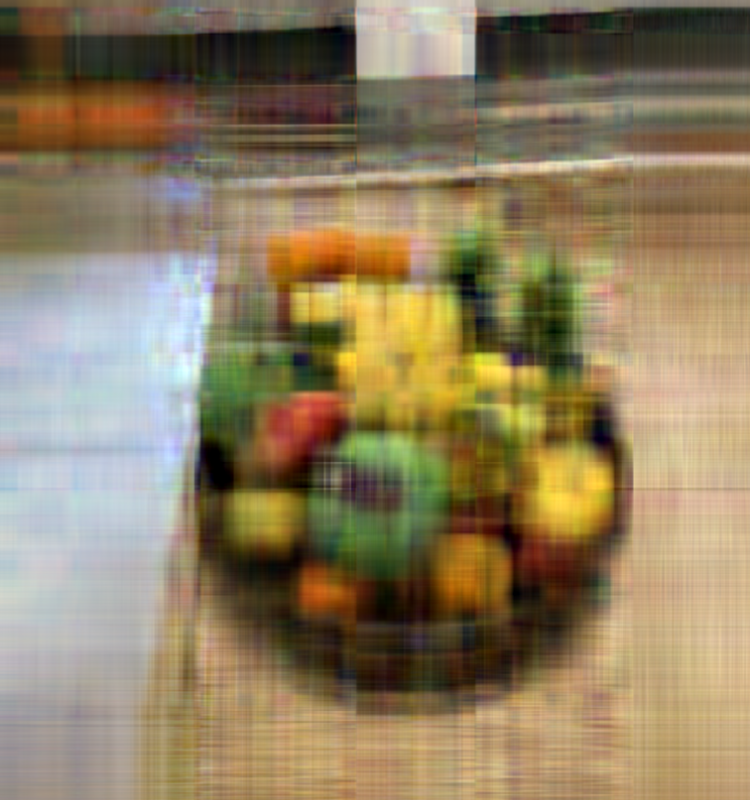
\includegraphics[width=0.8\textwidth]{ch2_figures/result_compression_fruit_10.png}
         \caption{Rank 10}
         \label{fig:compression_10}
     \end{subfigure}
     \centering
     \begin{subfigure}[b]{0.45\textwidth}
         \centering
         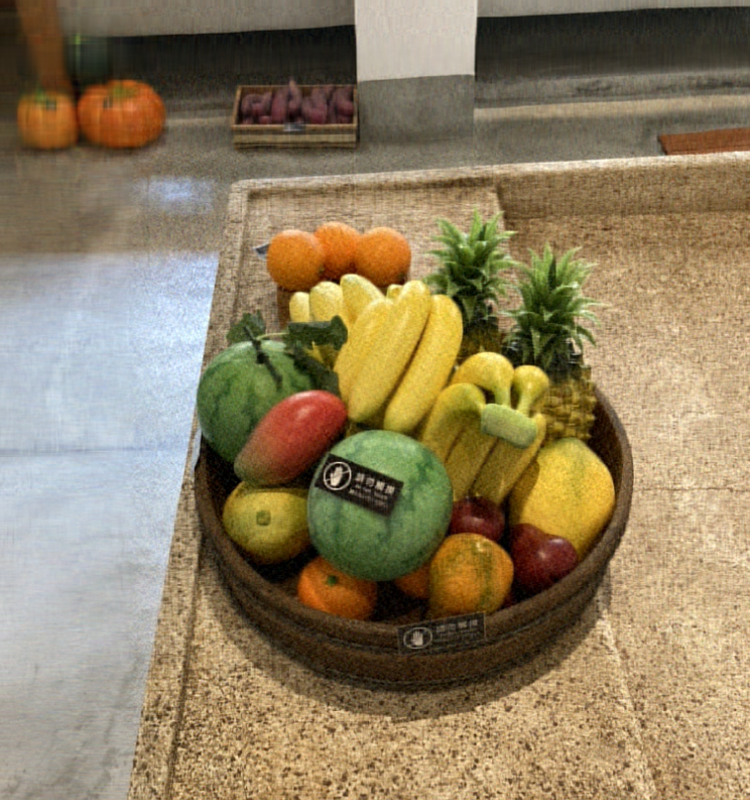
\includegraphics[width=0.8\textwidth]{ch2_figures/result_compression_fruit_100.png}
         \caption{Rank 100}
         \label{fig:compression_100}
     \end{subfigure}
     \hfill
     \begin{subfigure}[b]{0.45\textwidth}
         \centering
         
\includegraphics[width=0.8\textwidth]{ch2_figures/result_compression_fruit_200.png}
         \caption{Rank 200}
         \label{fig:compression_200}
     \end{subfigure}
     \caption{Compression results.}
     \label{fig:compressed_fruits}
\end{figure}

In this case, selecting 100 singular values gives an approximation matrix that closely resembles the original image matrix, enabling the identification of details within the image.

To assess the storage capacity saved through compression, we introduce the following definition.

\begin{definition}[Data Compression Ratio]
    The data compression ratio is the ratio between the size of uncompressed data and the size of compressed data. That is,
    \[ \text{Compression Ratio} = \frac{\text{Uncompressed Size}}{\text{Compressed Size}}. \]
\end{definition}

If the original image is a $m\times n$ matrix, then it contains $mn$ pixels. However, its rank-$k$ approximation can be stored in a space of size $k(m+n+1)$ pixels. The compression ratio of an image using SVD based compression is
\[ \frac{mn}{k(m+n+1)}. \]

To ensure that the compressed size is smaller than the uncompressed size, the compression ratio must be greater than 1. Therefore, the approximation rank $k$ must satisfy the following inequality:
\[ k < \frac{mn}{m+n+1}. \]

\begin{figure}
    \centering
    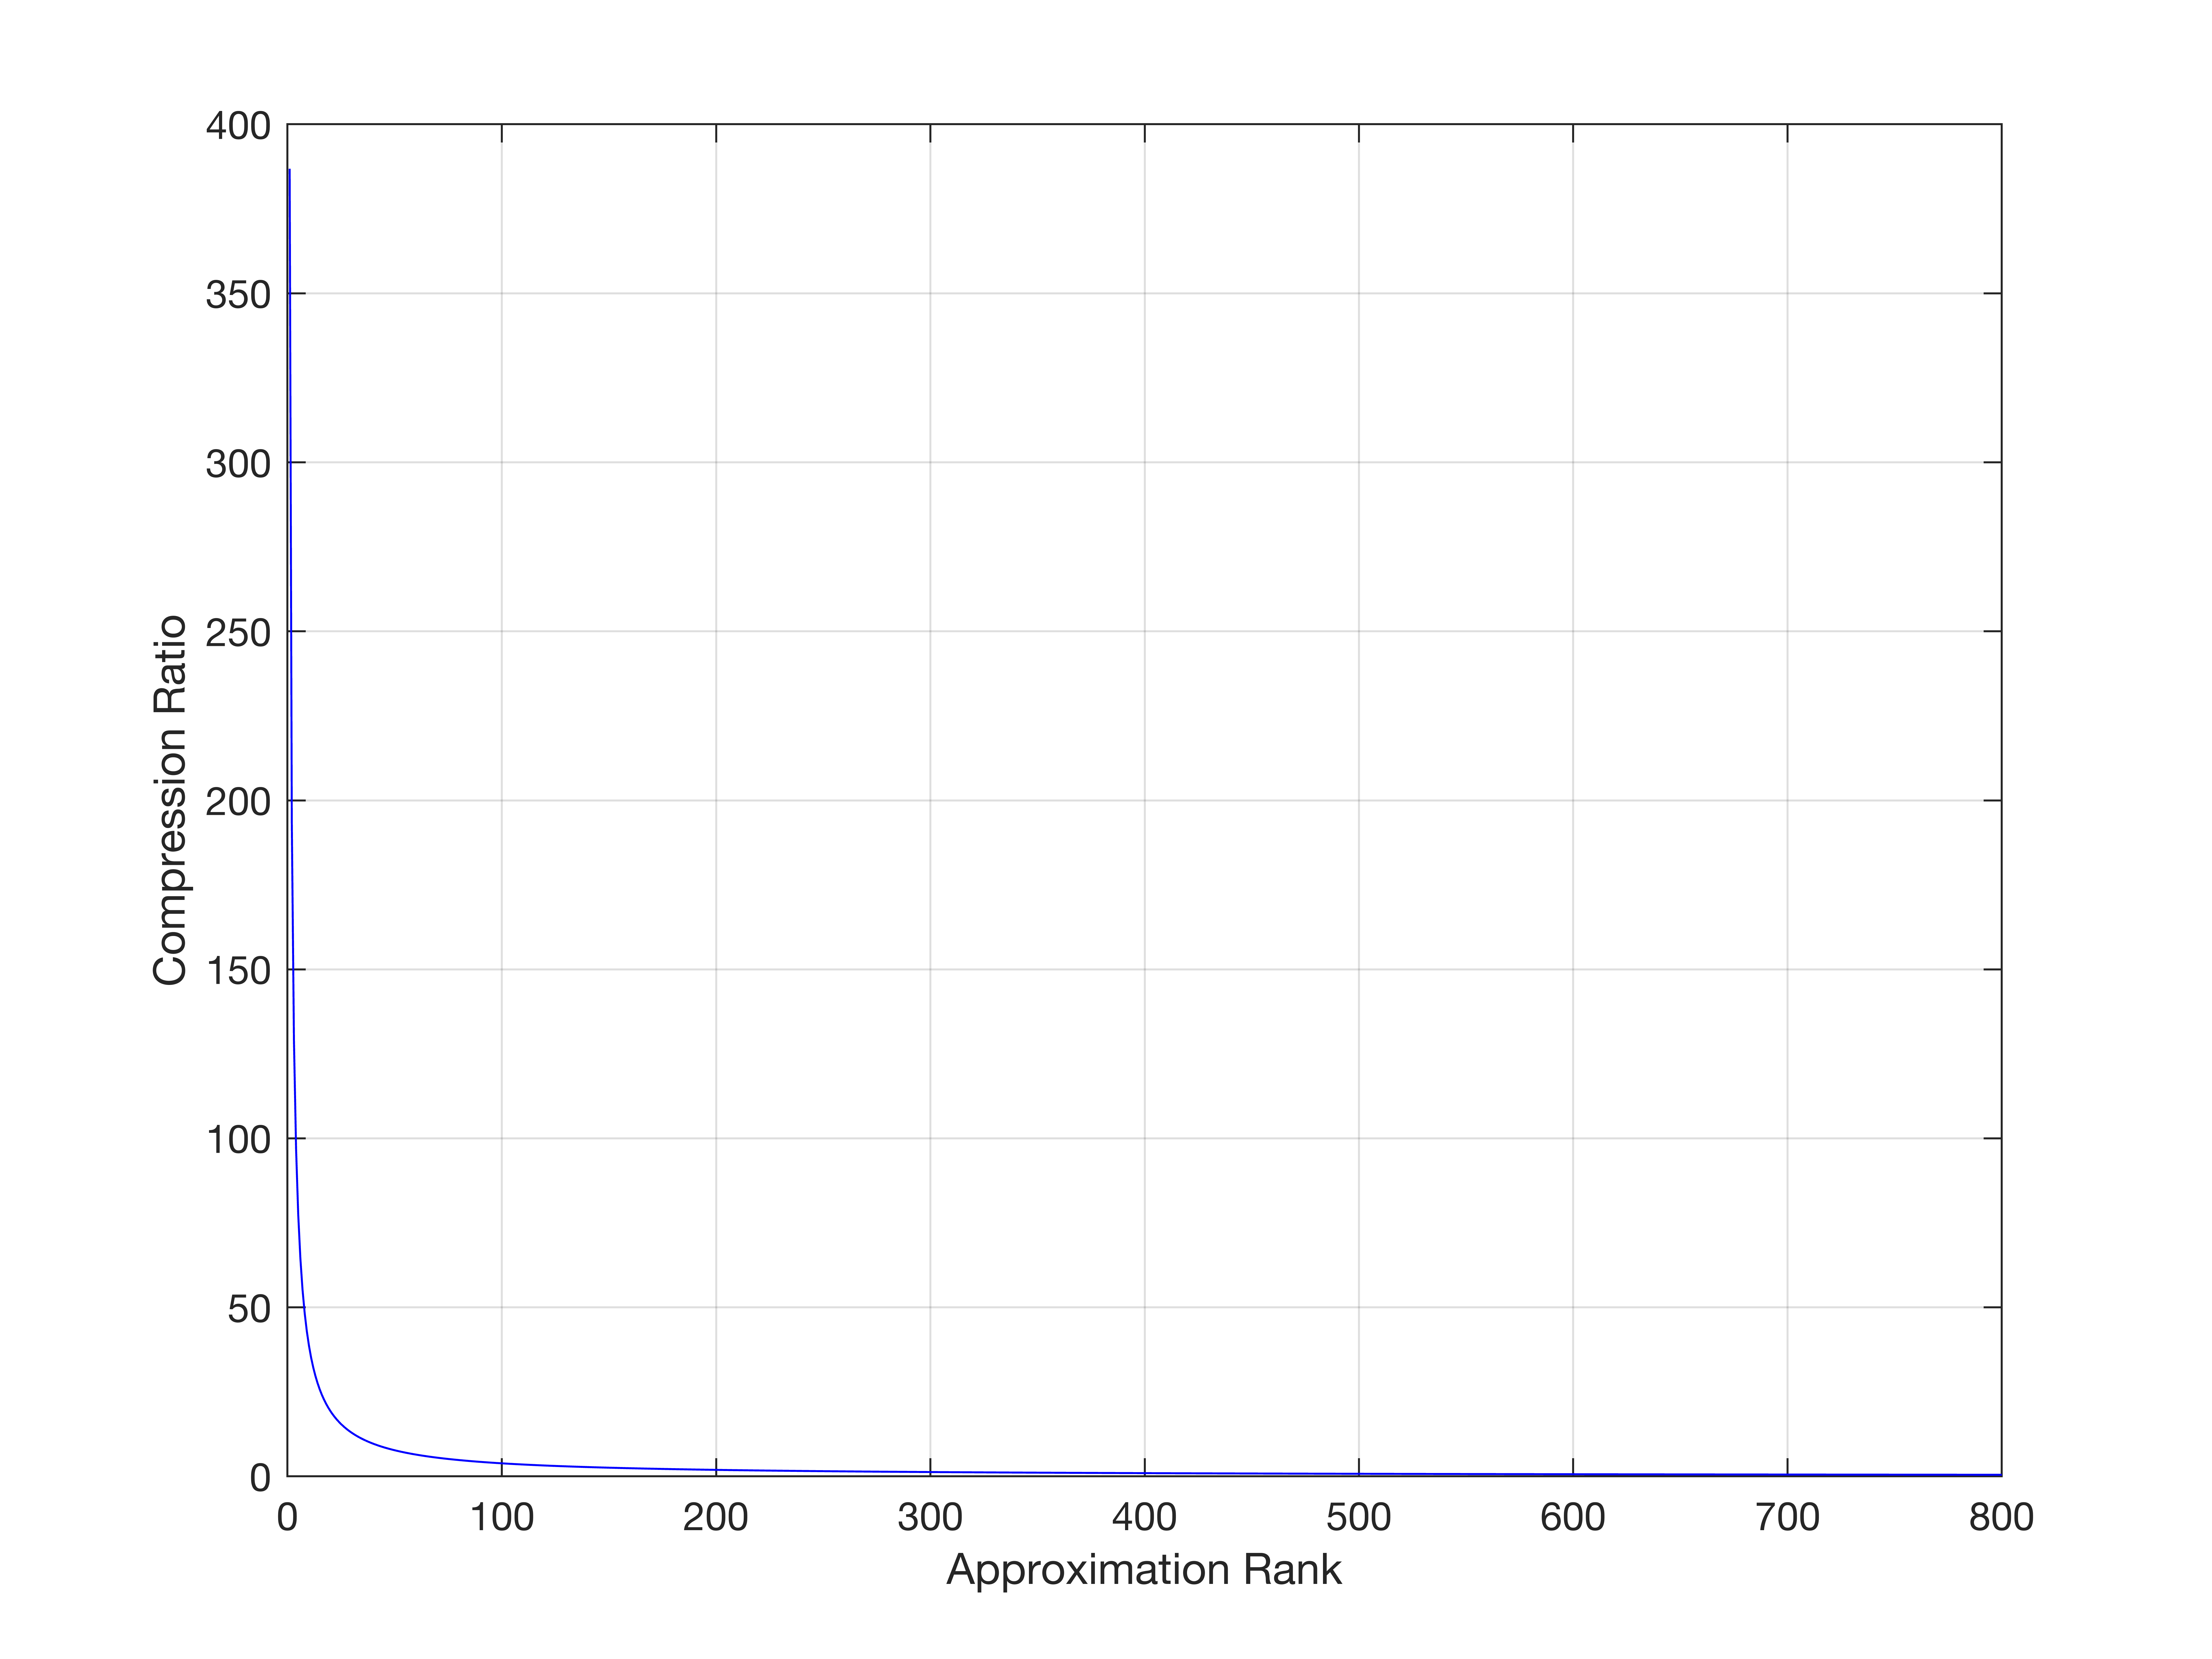
\includegraphics[width=0.8\textwidth]{ch2_figures/compression_ratio.png}
    \caption{Relation between approximation rank and compression ratio.}
    \label{fig:3}
\end{figure}

Figure \ref{fig:3} shows the relation between the approximation rank and the compression ratio of Figure \ref{fig:original_fruits}.

We employ two methods to assess the error between the compressed image and the original image. First, we utilize the magnitude of the singular values to determine the significance of the remaining values. Figure \ref{fig:singular_values} shows the relation between the approximation rank and the singular value of Figure \ref{fig:original_fruits}. The relation of each RGB layer is depicted in red, green, and blue, respectively. The singular values are displayed in a relative manner; that is, the relative singular value $\overline{\sigma_i}$ is defined by
\[ \overline{\sigma_i} = \frac{\sigma_i}{\sigma_1} \]
for each $i = 1,\ldots, \min\{m,n\}$.

\begin{figure}
    \centering
    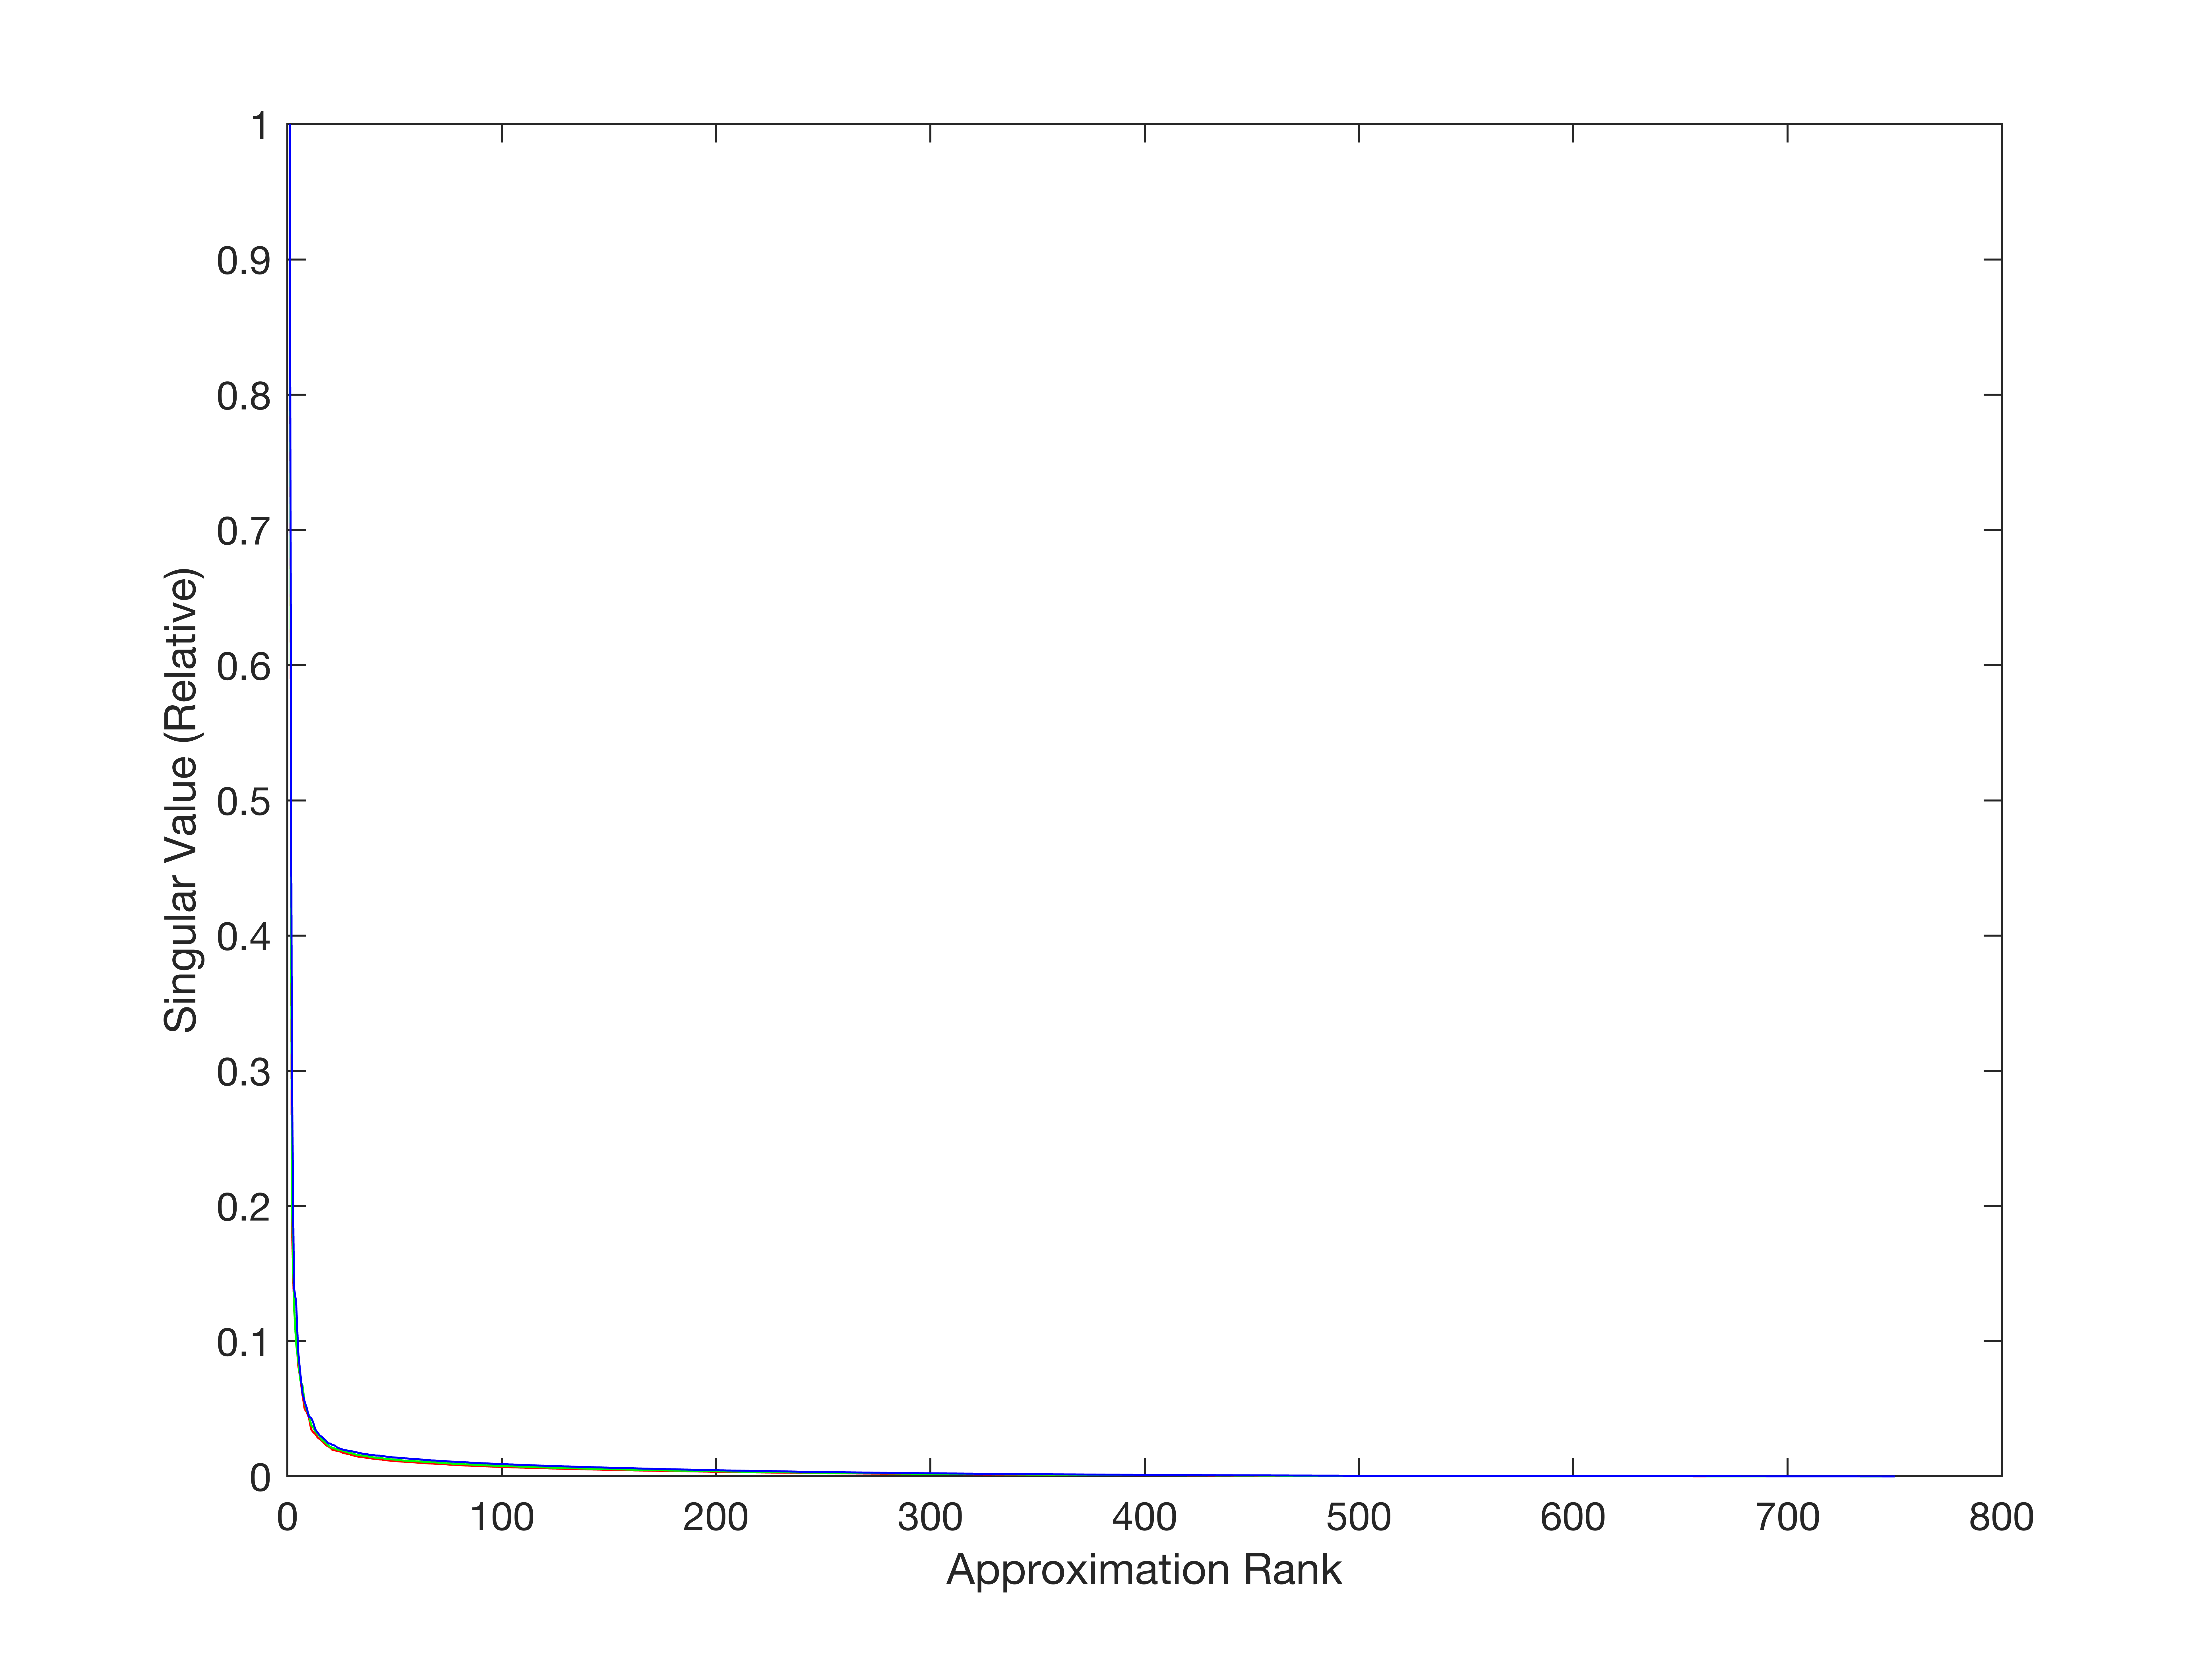
\includegraphics[width=0.8\textwidth]{ch2_figures/stat2.png}
    \caption{Relation between approximation rank and singular value.}
    \label{fig:singular_values}
\end{figure}

On the other hand, we use Frobenius norm to assess the error $\varepsilon_k$ between the compressed image and the original image:
\[ \varepsilon_k = \frac{\Vert A - \tilde{A}_k\Vert_F}{\Vert A\Vert_F}, \]
where $A$ is the original image matrix and $\tilde{A}_k$ is the rank-$k$ approximation of $A$. Figure \ref{fig:frob_norm} shows the relation between the approximation rank and the relative error.

\begin{figure}
    \centering
    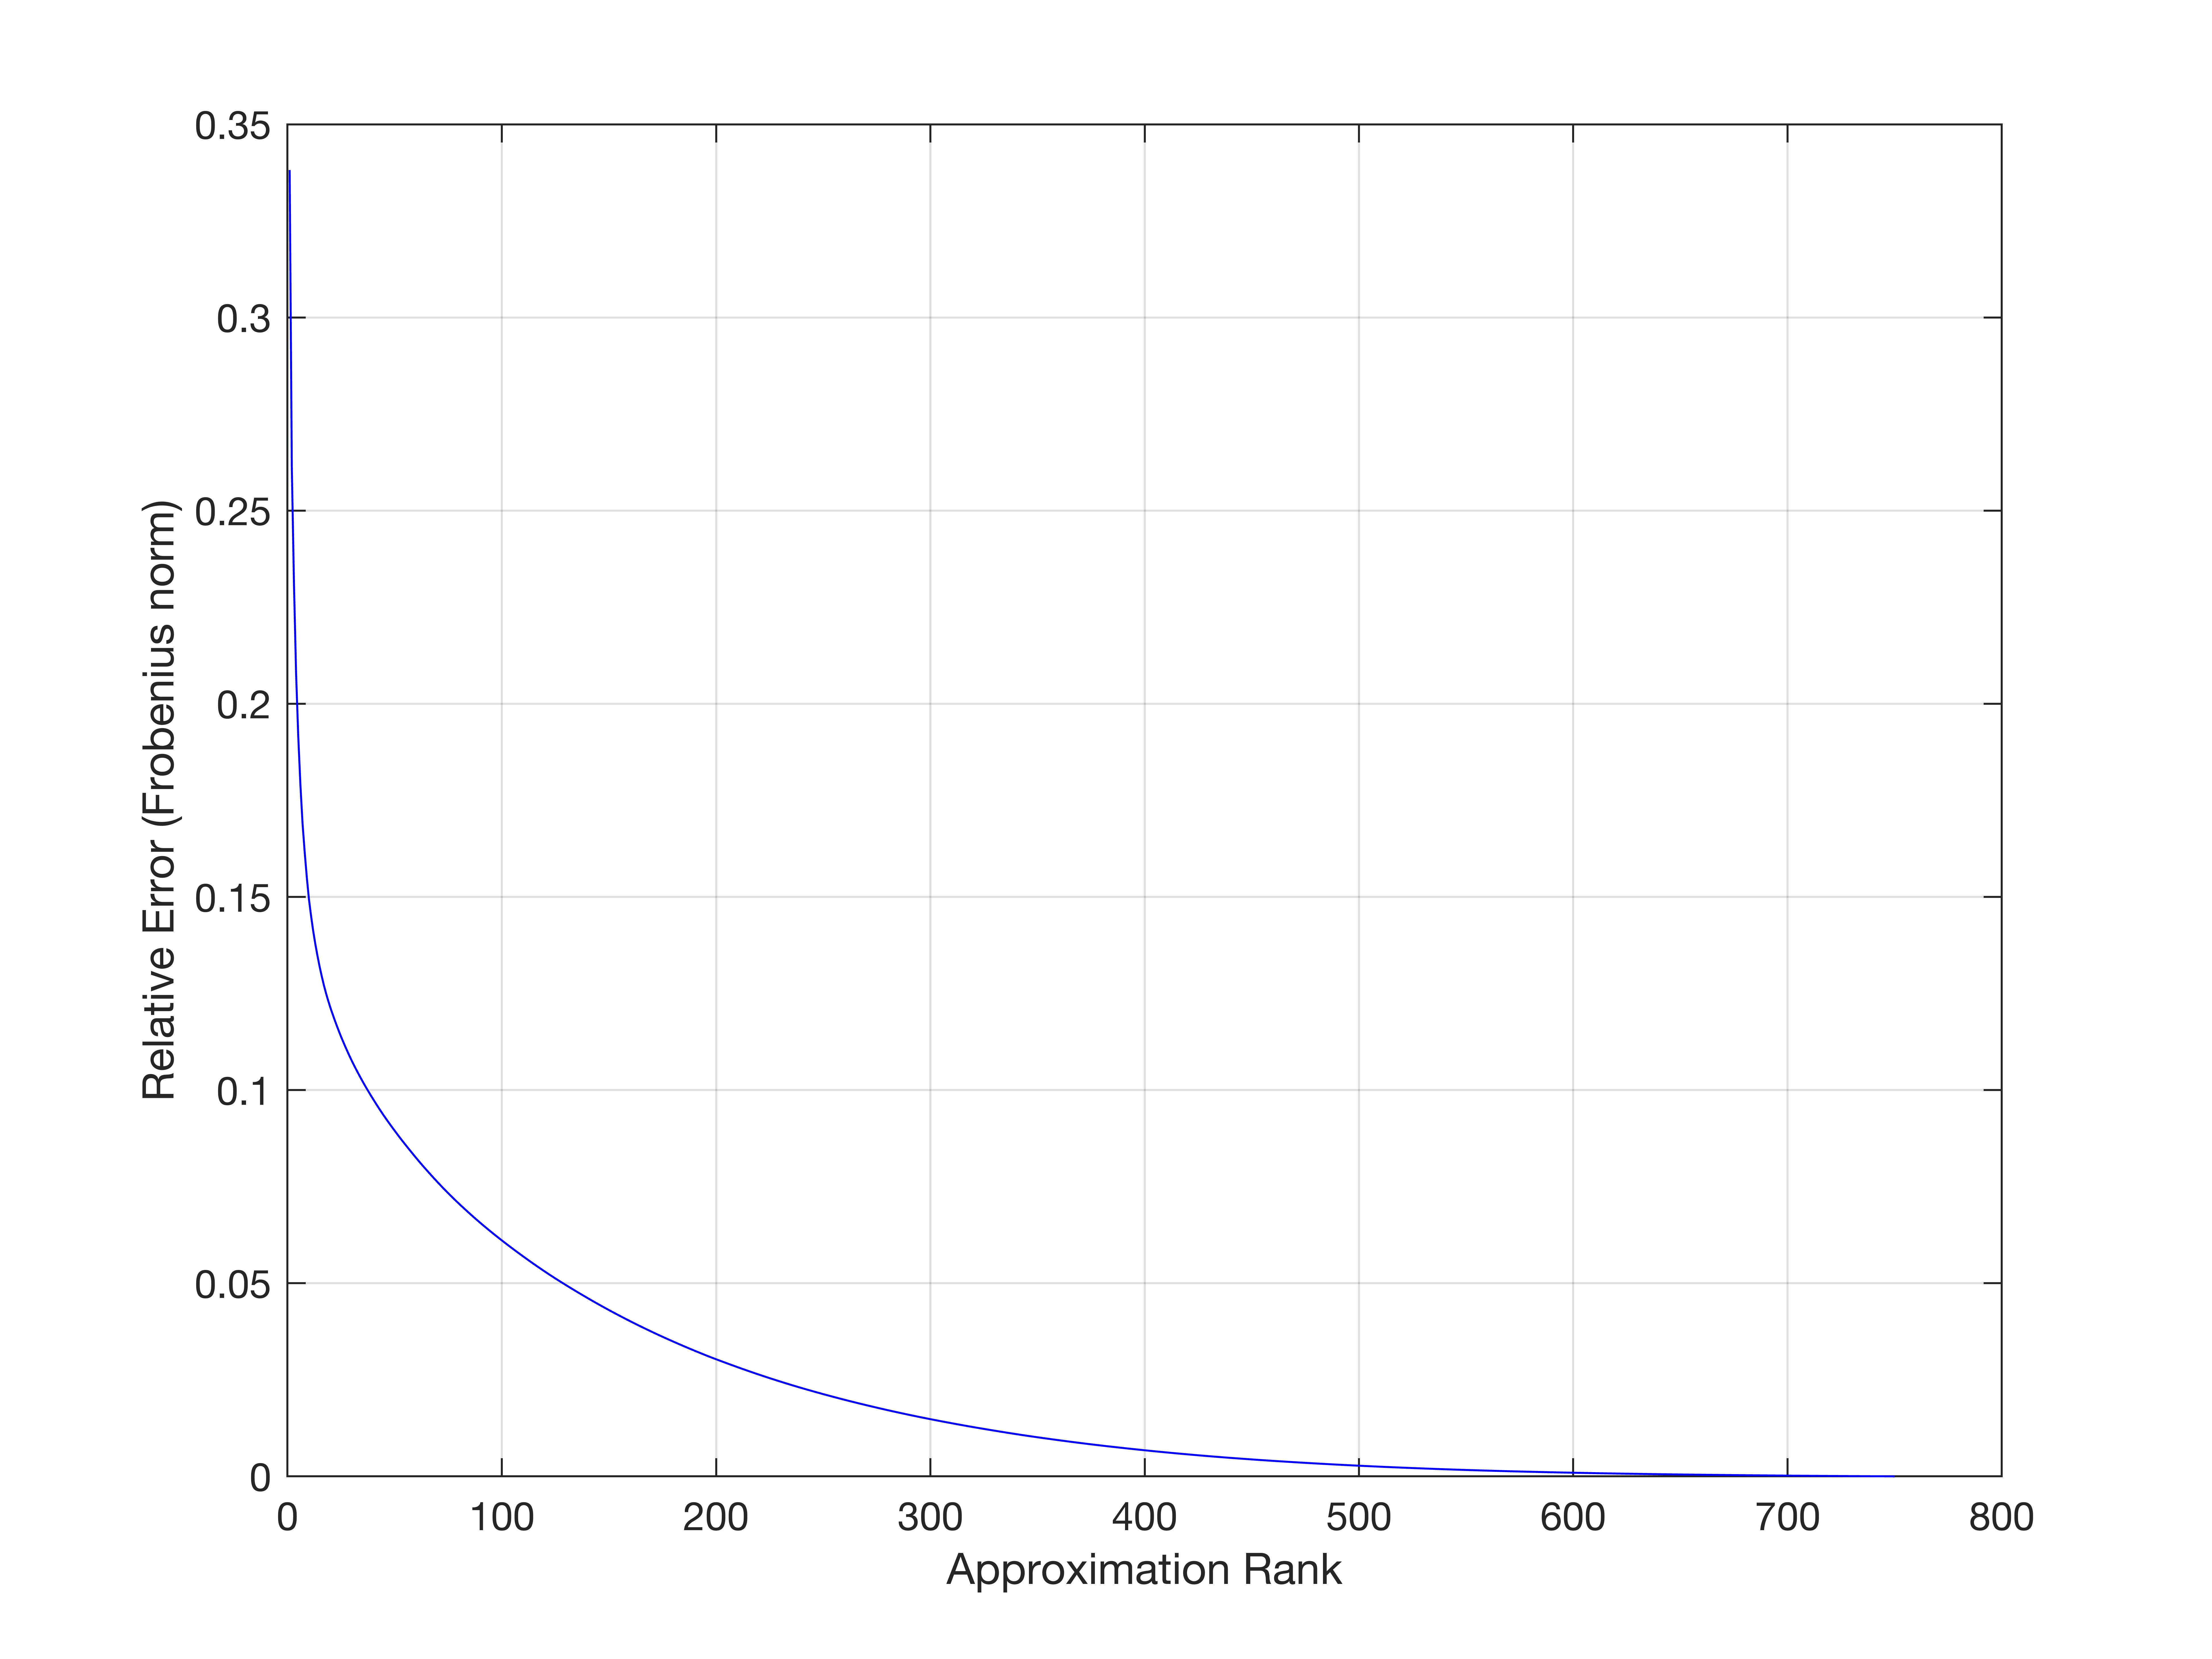
\includegraphics[width=0.8\textwidth]{ch2_figures/stat1.png}
    \caption{Relation between approximation rank and relative error.}
    \label{fig:frob_norm}
\end{figure}

\section{Live Photo Processing}
We find that Theorem \ref{thm:eym} allows us to effectively separate the substantial information of an image contained in the static background from the relatively sparse information of dynamic objects. While some information may be lost in this process, we have successfully removed the dynamic objects and obtained a static background. However, we further observe that the loss of certain information results in a blurred image. To address this issue, our aim is to eliminate the blurring and achieve clearer images.

\subsection{Magic Eraser} \label{subsec:magic_eraser}
Given a video with a resolution of $n\times m$, a frame rate of $f$ fps, and a duration of $t$ seconds, there are $ft$ frames in the video. Each frame consists of three channels of $m\times n$ matrices, assumed to be using RGB color encoding.

Let $R_k,G_k,B_k$ denote the R, G, B channel of the k-th frame of the video, respectively. Let $\mathbf{r}_k, \mathbf{g}_k, \mathbf{b}_k \in\mathbb{R}^{mn\times 1}$ be column vectors defined by
\begin{align*}
    (\mathbf{r}_k)_i = (R_k)_{(i-m\lfloor (i-1)/m\rfloor, \lceil i/m\rceil)}, \\
    (\mathbf{g}_k)_i = (G_k)_{(i-m\lfloor (i-1)/m\rfloor, \lceil i/m\rceil)}, \\
    (\mathbf{b}_k)_i = (B_k)_{(i-m\lfloor (i-1)/m\rfloor, \lceil i/m\rceil)}.
\end{align*}
Then let $\hat{R},\hat{G},\hat{B}\in\mathbb{R}^{mn\times ft}$ be matrices defined by
\[ \hat{R} = 
\begin{bmatrix}
    | & & | \\
    \mathbf{r}_1 & \cdots & \mathbf{r}_{ft} \\
    | & & |
\end{bmatrix}
, \quad\hat{G} = 
\begin{bmatrix}
    | & & | \\
    \mathbf{g}_1 & \cdots & \mathbf{g}_{ft} \\
    | & & | 
\end{bmatrix}
, \quad\hat{B} = 
\begin{bmatrix}
    | & & | \\
    \mathbf{b}_1 & \cdots & \mathbf{b}_{ft} \\
    | & & |
\end{bmatrix}
.
\]
We apply singular value decomposition to these matrices; that is,
\[ \hat{R} = U_R \Sigma_R V^\top_R, \quad
\hat{G} = U_G \Sigma_G V^\top_G,\quad
\hat{B} = U_B \Sigma_B V^\top_B.
\]
By choosing 
\[ \mathbf{r} = (\mathbf{u}_R)_1 (\sigma_R)_1 (v_R)_{11},
\quad \mathbf{g} = (\mathbf{u}_G)_1 (\sigma_G)_1 (v_G)_{11},
\quad \mathbf{b} = (\mathbf{u}_B)_1 (\sigma_B)_1 (v_B)_{11},
\]
where $\mathbf{r},\mathbf{g},\mathbf{b}\in\mathbb{R}^{mn\times 1}$ and let $\Tilde{R},\Tilde{G},\Tilde{B}\in\mathbb{R}^{m\times n}$ be matrices defined by
\[ \Tilde{R}_{ij} = \mathbf{r}_{i+m(j-1)}, \quad
\Tilde{G}_{ij} = \mathbf{g}_{i+m(j-1)}, \quad
\Tilde{B}_{ij} = \mathbf{b}_{i+m(j-1)}.
\]
Then the image $A = [\Tilde{R}\ \Tilde{G}\ \Tilde{B}]$ is close to the background without a moving object.

\subsection{Result}
We selected a video (Figure \ref{fig:video}) taken at NUKI Coffee near the main campus of National Taiwan Normal University. The video features two passersby walking in front of a static background. Our objective is to remove the passersby and obtain a clear background.

\begin{figure}[ht]
     \centering
     \begin{subfigure}[b]{0.3\textwidth}
         \centering
         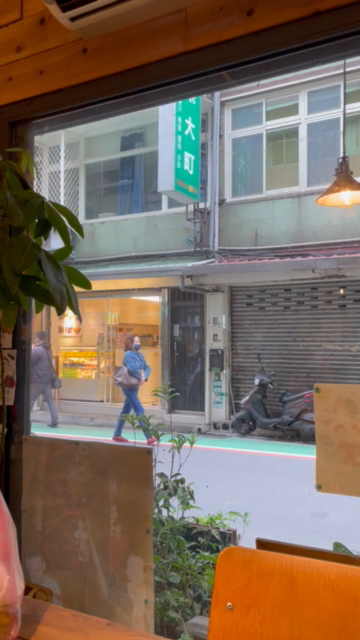
\includegraphics[width=\textwidth]{ch3_figures/video_1.png}
         \label{fig:video_1}
     \end{subfigure}
     \hfill
     \begin{subfigure}[b]{0.3\textwidth}
         \centering
         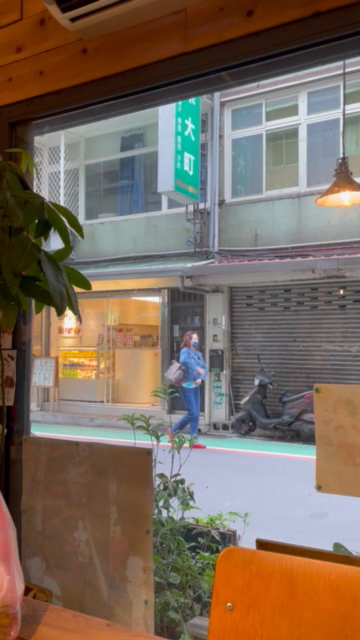
\includegraphics[width=\textwidth]{ch3_figures/video_2.png}
         \label{fig:video_2}
     \end{subfigure}
     \hfill
     \begin{subfigure}[b]{0.3\textwidth}
         \centering
         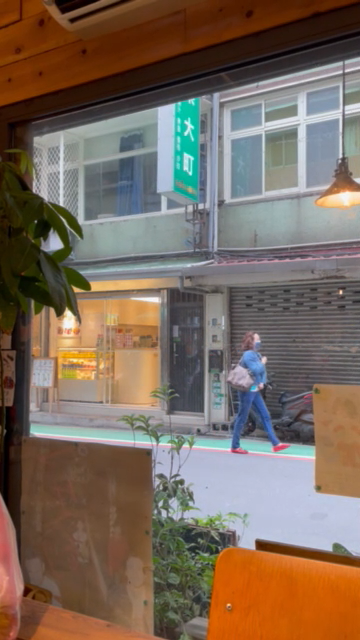
\includegraphics[width=\textwidth]{ch3_figures/video_3.png}
         \label{fig:video_3}
     \end{subfigure}
     \caption{A video of passersby walking against static background (232 frames).}
     \label{fig:video}
\end{figure}

\subsubsection{Analysis of Singular Values}
We found that in each $\hat{R},\hat{G},\hat{B}$ matrix, the largest singular value is much larger than the second largest singular value; that is,
\[ (\sigma_R)_1 \gg (\sigma_R)_2, \qquad
(\sigma_G)_1 \gg (\sigma_G)_2, \qquad
(\sigma_B)_1 \gg (\sigma_B)_2.
\]

\noindent
The five largest singular value of $\hat{R},\hat{G},\hat{B}$ are shown in Table \ref{tab:eraser_singular_values}.

\begin{table}[ht]
    \centering
    \begin{tabular}{@{}cccc@{}}
        \toprule
         & $\sigma_R$ & $\sigma_G$ & $\sigma_B$ \\
        \midrule
        $\sigma_1$ & $9.6994 \times 10^5$ & $8.6012 \times 10^5$ & $8.2226 \times 10^5$ \\
        $\sigma_2$ & $0.8230 \times 10^5$ & $0.7560 \times 10^5$ & $0.8202 \times 10^5$ \\
        $\sigma_3$ & $0.5283 \times 10^5$ & $0.4846 \times 10^5$ & $0.5020 \times 10^5$ \\
        $\sigma_4$ & $0.3061 \times 10^5$ & $0.2939 \times 10^5$ & $0.3028 \times 10^5$ \\
        $\sigma_5$ & $0.2139 \times 10^5$ & $0.1988 \times 10^5$ & $0.2074 \times 10^5$ \\
        \bottomrule
    \end{tabular}
    \caption{The singular values of $\hat{R}$, $\hat{G}$, and $\hat{B}$.}
    \label{tab:eraser_singular_values}
\end{table}

\noindent
It follows that the rank-1 approximation of $\hat{R},\hat{G},\hat{B}$ are close to the original matrices.

\subsubsection{BRISQUE}
The video we selected has a static background and dynamic foreground. We utilize singular value decomposition to extract the background image. Since we lack the original background image, we use a built-in function, \texttt{brisque()}, in MATLAB for a no-reference evaluation of the image quality.

In the work \cite{mittal2012no}, they introduced a distortion-generated blind/no-reference (NR) image quality assessment (IQA) model based on natural scene statistics operating in the spatial domain. The model is known as the Blind/No-Reference Image Spatial Quality Evaluator (BRISQUE), which uses statistics of local normalized brightness coefficients of the scene to quantify distortion. This method has very low computational complexity, making it ideal for real-time applications. Furthermore, its performance is independent of database content, and BRISQUE features can also be used for distortion identification.

The no-reference image quality score is returned as a non-negative scalar, typically falling within the range of [0, 100]. Lower scores indicate better perceptual image quality with respect to the input model.

\subsubsection{Result Evaluation}
Let $\mathbf{x}$ represent a result image matrix before reshaping of any color channels, namely $\mathbf{r},\mathbf{g},\mathbf{b}$ in Section \ref{subsec:magic_eraser},
\[ \mathbf{x}^{(1)} = \mathbf{u}_1 \sigma_1 v_{11},
\quad \mathbf{x}^{(2)} = \mathbf{u}_2 \sigma_2 v_{22},
\quad \mathbf{x}^{(\text{new})} = \mathbf{x}^{(1)} - \mathbf{x}^{(2)}.
\]
Let $A^{(1)}$, $A^{(2)}$, $A^{(\text{new})}$ be the result after reshaping $\mathbf{r},\mathbf{g},\mathbf{b}$, respectively. Upon visually observing that the image presented by $A^{(1)}$ exhibits slight shaking and blurriness, we found that the BRISQUE value for this image is 47.4178, which is not enough desirable. Similarly, the result for $A^{(2)}$ is more undesirable, and the image appears to consist mainly of structural lines of the house. To improve the image quality, we subtracted the result of $A^{(2)}$ from $A^{(1)}$ to obtain $A^{(\text{new})}$. As a result, the BRISQUE value improved, and the image became clearer. The images $A^{(1)}$, $A^{(2)}$, $A^{(\text{new})}$ are shown in Figure \ref{fig:video_after}.

\begin{table}[ht]
    \centering
    \begin{tabular}{@{}cccc@{}}
        \toprule
         & $A^{(1)}$ & $A^{(2)}$ & $A^{(\text{new})}$ \\
        \midrule
        \text{BRISQUE} & 47.4178 & 58.7426 & 39.6660 \\
        \bottomrule
    \end{tabular}
    \caption{The BRISQUE values of $A^{(1)}$, $A^{(2)}$, and $A^{(\text{new})}$.}
    \label{tab:brisque}
\end{table}

\begin{figure}[ht]
     \centering
     \begin{subfigure}[b]{0.3\textwidth}
         \centering
         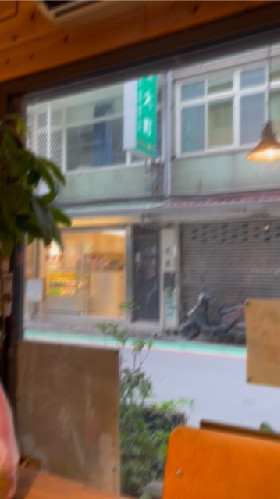
\includegraphics[width=\textwidth]{ch3_figures/video_after_1.png}
         \caption{$A^{(1)}$}
         \label{fig:video_after_1}
     \end{subfigure}
     \hfill
     \begin{subfigure}[b]{0.3\textwidth}
         \centering
         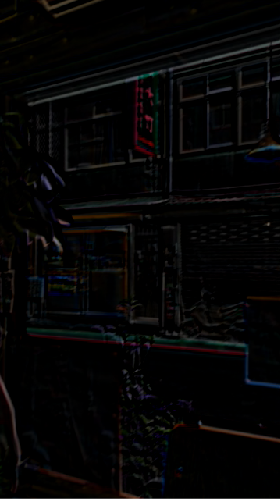
\includegraphics[width=\textwidth]{ch3_figures/video_after_2.png}
         \caption{$A^{(2)}$}
         \label{fig:video_after_2}
     \end{subfigure}
     \hfill
     \begin{subfigure}[b]{0.3\textwidth}
         \centering
         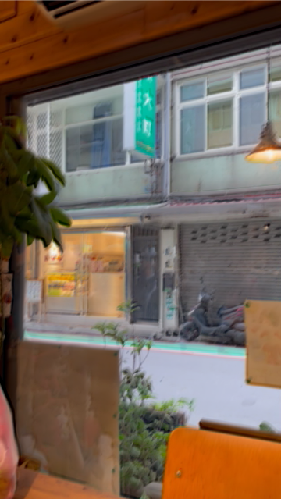
\includegraphics[width=\textwidth]{ch3_figures/video_after_3.png}
         \caption{$A^{(\text{new})}$}
         \label{fig:video_after_3}
     \end{subfigure}
     \caption{The result image by selecting different $\mathbf{x}$.}
     \label{fig:video_after}
\end{figure}

\section{Conclusion}
In this research, we utilize singular value decomposition and select an appropriate number of singular values. This not only helps preserve important details while using less storage, but also achieves the effect of image compression. In addition, we removed dynamic objects from the video while retaining static background information. Among them, static background information has the highest proportion, while dynamic objects are regarded as secondary information.

However, our approach is not without its limitations. Firstly, it may face difficulties when dealing with extremely large matrix operations caused by longer videos, which could limit its practical feasibility. Secondly, in different video scenarios, such as when dynamic objects occupy a substantial portion of the video, the effectiveness of removal becomes challenging due to the vast amount of information contained in these dynamic objects.

Future work includes exploring methods to retain dynamic objects in Section \ref{subsec:magic_eraser} and replacing the background. Additionally, we can consider incorporating other techniques, such as feature matching, to further enhance the final deblurring effect.

\section*{Appendix}
The codes and files are available on \href{https://github.com/lemonade0715/1121_scientific_computation}{GitHub}.

\subsubsection*{\texttt{test\_norms.m}}
\begin{lstlisting}[language=Matlab, style=mystyle]
% test_norms.m

norm_type_enum = {1, 2, inf, 'fro'};
norm_name_enum = {'1-', '2-', 'Infinity ', 'Frobenius '};
init = 500;
samples = 10;
stats = zeros(samples, 4);

for i=1:length(norm_name_enum)
    fprintf("\n[%snorm]\n", norm_name_enum{i});
    for j=1:samples
        fprintf("Calculating sample %d...\n",j);
        A = rand(init*j,init*j);
        tic;
        norm(A, norm_type_enum{i});
        stats(j,i) = toc;
    end
end
disp(stats);
\end{lstlisting}

\subsubsection*{\texttt{stat.m}}
\begin{lstlisting}[language=Matlab, style=mystyle]
% stat.m

% Input image and define norm type
image_path = './result/result_compression_fruit_orig.png';
norm_type = 'fro';
norm_name = 'Frobenius norm';
[~, img_name, img_ext] = fileparts(image_path);
img = imread(image_path);

% Get matrix infos
[m,n,num_layers] = size(img);
sv_num = min(m,n);
errors = zeros(1, sv_num);

% SVD
orig_norm = norm(double(img), norm_type);
[U, S, V] = pagesvd(double(img), "econ");
V_conj = pagetranspose(V);

% Calculate the relative errors
result = zeros(m, n, num_layers);
for rank = 1:sv_num
    fprintf("Calculating rank = %d...\n", rank);
    result = result + S(rank,rank,:) .* U(:,rank,:) .* V_conj(rank,:,:);
    errors(1,rank) = norm(double(result)-double(img), norm_type) / orig_norm;
end

% Plot the values
index_vector = 1:min(m,n);
figure;
plot(index_vector, errors(:), 'b-');
xlabel('Approximation Rank');
ylabel(['Relative Error (', norm_name, ')']);
grid on;
figure;
plot(index_vector, diag(S(:,:,1)) ./ S(1,1,1), 'r-', index_vector, diag(S(:,:,2)) ./ S(1,1,2), 'g-', index_vector, diag(S(:,:,3)) ./ S(1,1,3), 'b-');
xlabel('Approximation Rank');
ylabel('Singular Value (Relative)');
\end{lstlisting}

\subsubsection*{\texttt{image\_compression.m}}
\begin{lstlisting}[language=Matlab, style=mystyle]
% image_compression.m

% Set Image Path and Rank
imageFilePath = './result/result_compression_fruit_orig.png';
sv_num = 5;

% Get Image Info
info = imfinfo(imageFilePath);
img = imread(imageFilePath);
[img_size_x, img_size_y, channels] = size(img);
fprintf('image size: %dx%d, channel=%d\n', img_size_x, img_size_y, channels);
sv_total = sv(double(img(:,:,1)));
fprintf('singular value: %d/%d\n', sv_num, sv_total);
comp_ratio = (img_size_x * img_size_y) / (sv_num * (img_size_x + img_size_y + 1));
fprintf('compression ratio: %f\n', comp_ratio);

% Calculate the Low-Rank Approximation
layer = zeros(img_size_x, img_size_y, channels);
for i=1:channels
    layer = double(img(:,:,i));
    result = lr_approx(layer, sv_num);
    img(:,:,i) = uint16(result);
end

% Output and show the result
imshow(img);
[~, imageName, imageExt] = fileparts(imageFilePath);
if ~exist("result", 'dir')
    mkdir("result");
end
imwrite(img, sprintf("./result/result_compression_%s_%d%s", imageName, sv_num, imageExt), "png");

% Get Amount of Non-Zero Singular Values
function result = sv(A)
    [~, S, ~] = svd(A, "econ");
    [result, ~] = size(find(diag(S) ~= 0));
end

% Low Rank Approximation
function result = lr_approx(A, sv_num)
    [m, n] = size(A);
    [U, S, V] = svd(A, "econ");
    V_conj = V';
    for rank=1:sv_num
        result = zeros([m, n]);
        for j=1:rank
            result = result + S(j,j) * U(:,j) * V_conj(j,:);
        end
    end
end
\end{lstlisting}

\subsection*{\texttt{video.m}}
\begin{lstlisting}[language=Matlab, style=mystyle]
% video.m
obj = VideoReader("walk.mp4");
numFrames = obj.NumFrames;
%
init_directory();
for i=1:numFrames
    frame = read(obj,i);
    show_read_frame_progress(i,numFrames,10);
    imwrite(frame,strcat("./photos/shark_",num2str(i),'.png'),'png');
end
%}

[x,y,z] = size(imread("./photos/shark_1.png"));
X = zeros(x,y,z,"uint8");
frame_sep = 6;
for channel=1:z
    A = zeros(x*y, ceil(numFrames/frame_sep));
    frame_count = 1;
    for i=1:frame_sep:numFrames
        img = imread(sprintf("./photos/shark_%d.png",i));
        fprintf("Reshaping frame %d of channel %d...\n", i, channel);
        A(:,frame_count) = reshape(img(:,:,channel),[],1);
        frame_count = frame_count + 1;
    end
    fprintf("Complete!\n\n");
    fprintf("Starting singular value decomposition of channel %d...\n", channel);
    [U,S,V] = svd(A,'econ');
    fprintf("Reshaping channel %d of the image...\n", channel);
    disp("Singular Values:");
    disp(diag(S));
    X(:,:,channel) = uint8(reshape(U(:,1) .* S(1,1) .* V(1,1), x, y));
    fprintf("Complete!\n\n");
end
disp("Complete!");
imshow(X);

function init_directory(~)
    disp("Initializing directory './photos/'...");
    delete ./photos/*.png;
    fprintf("Complete!\n\n");
end

function show_read_frame_progress(curr,total,sep)
    if (mod(curr,sep) == 1)
        if (curr+sep-1 < total)
            fprintf("Writing frame %d-%d", curr, curr+sep-1);
            fprintf(" to './photos/'...\n");
        else
            fprintf("Writing frame %d-%d", curr, total);
            fprintf(" to './photos/'...\n");
            fprintf("Complete!\n\n");
        end        
    end
end
\end{lstlisting}

\nocite{*}
\printbibliography

%%%%%%%%%%%%%%%%%%%%%%%%%%%%%%
\end{document}